\documentclass{article}

\usepackage{neurips_2026}
\usepackage[utf8]{inputenc} % allow utf-8 input
\usepackage[T1]{fontenc}    % use 8-bit T1 fonts
\usepackage{hyperref}       % hyperlinks
\usepackage{url}            % simple URL typesetting
\usepackage{booktabs}       % professional-quality tables
\usepackage{amsfonts}       % blackboard math symbols
\usepackage{nicefrac}       % compact symbols for 1/2, etc.
\usepackage{microtype}      % microtypography
\usepackage[table]{xcolor}  % colors and table cell backgrounds
\usepackage{amsmath}
\usepackage{cleveref}
\usepackage{multirow}
\usepackage{graphicx}      % for \includegraphics
\usepackage{wrapfig}
\newcommand{\yy}[1]{\textcolor{orange}{[Yujun:\ #1]}}
\title{	
What Makes Language Models Intelligent? Small-World Structure in Attention Head Networks}

\author{ }


\begin{document}


\maketitle


\begin{abstract}

Understanding what internal structures distinguish more capable large language models (LLMs) from less capable ones remains an open challenge. Inspired by neuroscience, we investigate whether LLMs exhibit small-world functional organization and whether this organization is associated with reasoning ability. We construct functional graphs over attention heads using activation similarity on fluid reasoning tasks, and find that a stronger small-world index (SWI) is consistently associated with better performance on fluid intelligence benchmarks across models. To validate the functional importance of this finding, we apply it to LLM pruning, where the goal is to preserve SWI during pruning and evaluate whether the resulting pruned models maintain strong performance. Since SWI is a graph-level measure, we further map it to local model structure by deriving node-level scores based on the two defining properties of small-world networks. Specifically, core scores quantify within-community connectivity related to local clustering, while bridge scores quantify cross-community connectivity related to short communication paths. Building on these local roles, we introduce our pruning method, Small-World Allocation (SWA), which aggregates node-level structural priorities to guide sparsity allocation across layers and attention heads. Experiments show that SWA better preserves both small-world organization and model performance, achieving up to a 20.01\% improvement over state-of-the-art pruning baselines. These results suggest that small-world functional organization is a measurable structural principle associated with LLM reasoning capability.
\end{abstract}




\section{Introduction}

%q1: tale 1 of different level. but the setup is in exp. q2: cka vs cca. from high level why cka does not work. say from ns. when 1d in ns, svcca is same as pearson. need to check








% what make llm intelligent? An invest into stuctu property of atten heads.

% chara of a more intelligent llm. 
% llm has great ability, even close to human. we do not know what llm is a smarter one. to get smarter llm, we do not have a guidance. this is the goal.


% considering the close of human brain and llm, in ns xxx. 
% cv network has 
% inspired from ns, 
% goal: info smarter llm

% we compare llm and brain. inspired by ns, we study xxx. we focus on swi, and its correlation w.r.t intelligence. we find it is same as human brain. indicates that llm' head activation. based on the finding. prune can add to 2-3 sentences. pruneing to preserve the swi metric. this verify the impact of the metrics.




% figure, draw multiple layers
% change the circle to different color, give path a line

% change figure 1 to two figures
% make swi-perf with real data
% stack the two figures.


% prelim: 1. define swi. different quantity. how it used in ns, and the conclusion in ns.
% 2. notation

% key insights have a new section. 1. show how the graph is built (what data is used, what factor is tested by the data) 
% 2. and the exp results. 

% application driven by our finding: say two scores and used in pruning.
% goal: maintain swi. as considering pruning, global compute has issue. rather than comuting, we define xxx scores. potentially preserve swi. they can support head/layer.
% ADD!!!! core/bridge score illustration

% exp: 1. prove scors can preserve swi. ADD LLAMA.
% 2. pruning model results
% 3. intelli results
% 4. abl


% Large language models (LLMs) have demonstrated increasingly strong reasoning abilities, approaching human-level performance on a growing range of benchmarks \cite{leon2025gpt, liu2025deepseek, gardinazzi2024persistent}. Understanding why some models reason better than others is therefore central to explaining and improving model intelligence. Benchmarks help measure this difference by evaluating model behavior across diverse reasoning tasks \cite{wang2024mmlu, kaplan2020scaling, schaeffer2023emergent}. Moving from measurement to explanation requires identifying the internal organization that give rise to stronger reasoning ability \cite{liang2022holistic, rai2024practical}. This motivates a central question: what structural properties distinguish more capable LLMs from less capable ones?

Large language models (LLMs) have demonstrated increasingly strong reasoning abilities, approaching human-level performance on a growing range of benchmarks \cite{leon2025gpt, liu2025deepseek, gardinazzi2024persistent}. Existing benchmarks measure these abilities by evaluating model behavior across diverse reasoning tasks \cite{wang2024mmlu, kaplan2020scaling, schaeffer2023emergent}. However, behavioral evaluation alone does not explain why some models reason better than others. To move from measuring reasoning performance to understanding its underlying mechanisms, we need to examine how reasoning capability is encoded in the model itself. In particular, the neural activation
%\yy{you said neural activations are more accurate?} 
of an LLM may exhibit structural properties that reflect how the model organizes and composes information for reasoning \cite{zhang2024interpreting, rai2024practical}. This motivates a central question: what structural properties of internal organization distinguish more capable LLMs from less capable ones?
%on fluid intelligence benchmarks, which emphasize abstract reasoning and rule generalization \cite{yang2025truly, wu2025understanding}?



Existing structural analyses provide useful starting points. You et al. model neural architectures as relational graphs, where nodes denote computational units and edges encode message-passing connectivity, and show that architecture-level topology is predictive of generalization performance in computer vision models \cite{you2020graph}. However, this graph representation is determined by the architecture itself and is therefore largely independent of the training data and optimization process. Since reasoning ability is shaped by data-dependent training and can vary across models with similar architectures, architecture-level topology alone cannot explain why some trained LLMs reason better than others. Moreover, these analyses have primarily been applied to vision models, leaving open how to characterize the internal organization of trained LLMs.
% However, because this graph representation is specified by the network architecture rather than inferred from learned, data-dependent model behavior\yy{just say it is irrelevant to the training data and the optimization process, thus cannot be used to measure the reasoning abilities of the LLMs which is data- and training- dependent. also mention they only apply to vision models, not LLMs}, it does not capture the organization that emerges in a particular trained model. 
Another line of work studies trained models through the spectra of their learned weight matrices. Grounded in random matrix theory and Heavy-Tailed Self-Regularization Theory \cite{hu2025eigenspectrum, lu2024alphapruning}, these methods analyze empirical spectral densities and shape metrics, such as spectral decay and heavy-tailed behavior, to characterize training quality, generalization behavior, and pruning sensitivity~\cite{martin2021predicting, yang2023test}.
These spectral methods suggest that internal structure is informative, but they leave open whether it is associated with intelligence-related reasoning performance and provide limited insight into structural organization.
% These spectral methods suggest that internal structure is informative, but they leave open whether such structure associated with intelligence-related reasoning performance and provide limited insights on structural organization.
% \yy{you can also mention they are spectral methods, providing limited insights on structural organization and development of methods for structural intervention} 
To investigate the functional organization of LLMs, we draw inspiration from neuroscience, where intelligence has been linked to the topology and efficiency of functional brain networks \cite{langer2012functional, barbey2018network}. Functional brain networks treat anatomical regions of interest (ROIs) as nodes and define edges by statistical dependencies computed over their activity time series, rather than by anatomical connectivity alone. Prior studies have linked intelligence-related performance to functional brain network efficiency, often characterized by small-world properties such as high clustering coefficient and short path length \cite{langer2012functional, rosenberg2020functional}. Such organization is thought to support efficient information processing by combining densely connected local neighborhoods with short communication paths between distant regions \cite{latora2001efficient, bassett2017small}. Motivated by these findings, we ask whether activations in LLMs reveal analogous graph signatures associated with intelligence-related reasoning performance.


% Spectral properties of weight matrices have been linked to trained model quality \cite{hu2025eigenspectrum, lu2024alphapruning}, and graph-based analyses show that architectural connectivity can influence the predictive performance of deep neural networks \cite{you2020graph}.
% However, these studies mainly characterize weight statistics or architectural connectivity, and do not directly explain what internal structures distinguish LLMs that perform better on intelligence-related reasoning tasks.
% To seek such principles, we turn to neuroscience, where intelligence has been linked to the organization of functional brain networks \cite{langer2012functional, barbey2018network}. 
% In particular, higher intelligence-test performance has been associated with stronger small-world organization, reflected by higher local clustering and shorter characteristic path lengths \cite{langer2012functional, rosenberg2020functional}. 
% This topology supports efficient information processing through dense local connectivity and short communication paths across distant brain regions \cite{latora2001efficient, bassett2017small}. 
% This raises a natural question: do LLMs exhibit analogous internal structures that relate to their intelligence?


% \yy{Prior work has begun to study model capability through the lens of internal structure. You et al. model neural architectures as relational graphs, where nodes denote computational units and edges encode message-passing connectivity, and show that architecture-level topology is predictive of generalization performance in computer vision models \cite{you2020graph}. However, because their graph representation is determined by the network architecture rather than learned from data and optimization, it does not capture training- and data-dependent properties of a particular model. Moreover, their analysis focuses on vision models, leaving open how to characterize graph structure in the learned weights of LLMs and how such structure relates to reasoning ability. A complementary line of work studies trained models through the spectra of their learned weight matrices. Grounded in random matrix theory and Heavy-Tailed Self-Regularization, these methods analyze empirical spectral densities and associated shape metrics, such as spectral decay and heavy-tailed behavior, and relate them to model quality, training state, generalization, or pruning sensitivity \cite{hu2025eigenspectrum, lu2024alphapruning}. [cite a 2 more works here] While this line of work shows that learned weights contain informative signatures of trained models, it characterizes weights primarily through spectral matrix statistics. In contrast, we ask whether learned LLM weights exhibit graph organization that is associated with intelligence-related reasoning performance. }

% \yy{To guide the search for such organization, we draw inspiration from neuroscience, where intelligence has been linked to the topology and efficiency of functional brain networks \cite{langer2012functional, barbey2018network}. Functional brain networks represent brain regions as nodes and functional interactions, typically estimated from statistical dependencies in neural activity, as edges. Prior studies have linked intelligence-related performance to functional brain network efficiency, often characterized through small-world properties such as high clustering coefficient and short path length \cite{langer2012functional, rosenberg2020functional}. Such organization is thought to support efficient information processing by combining densely connected local neighborhoods with short communication paths between distant regions \cite{latora2001efficient, bassett2017small}. Motivated by these findings, we ask whether graph signatures in learned LLM weights are also associated with their reasoning capability.}


\begin{figure}%{r}{0.58\textwidth}
    \centering
    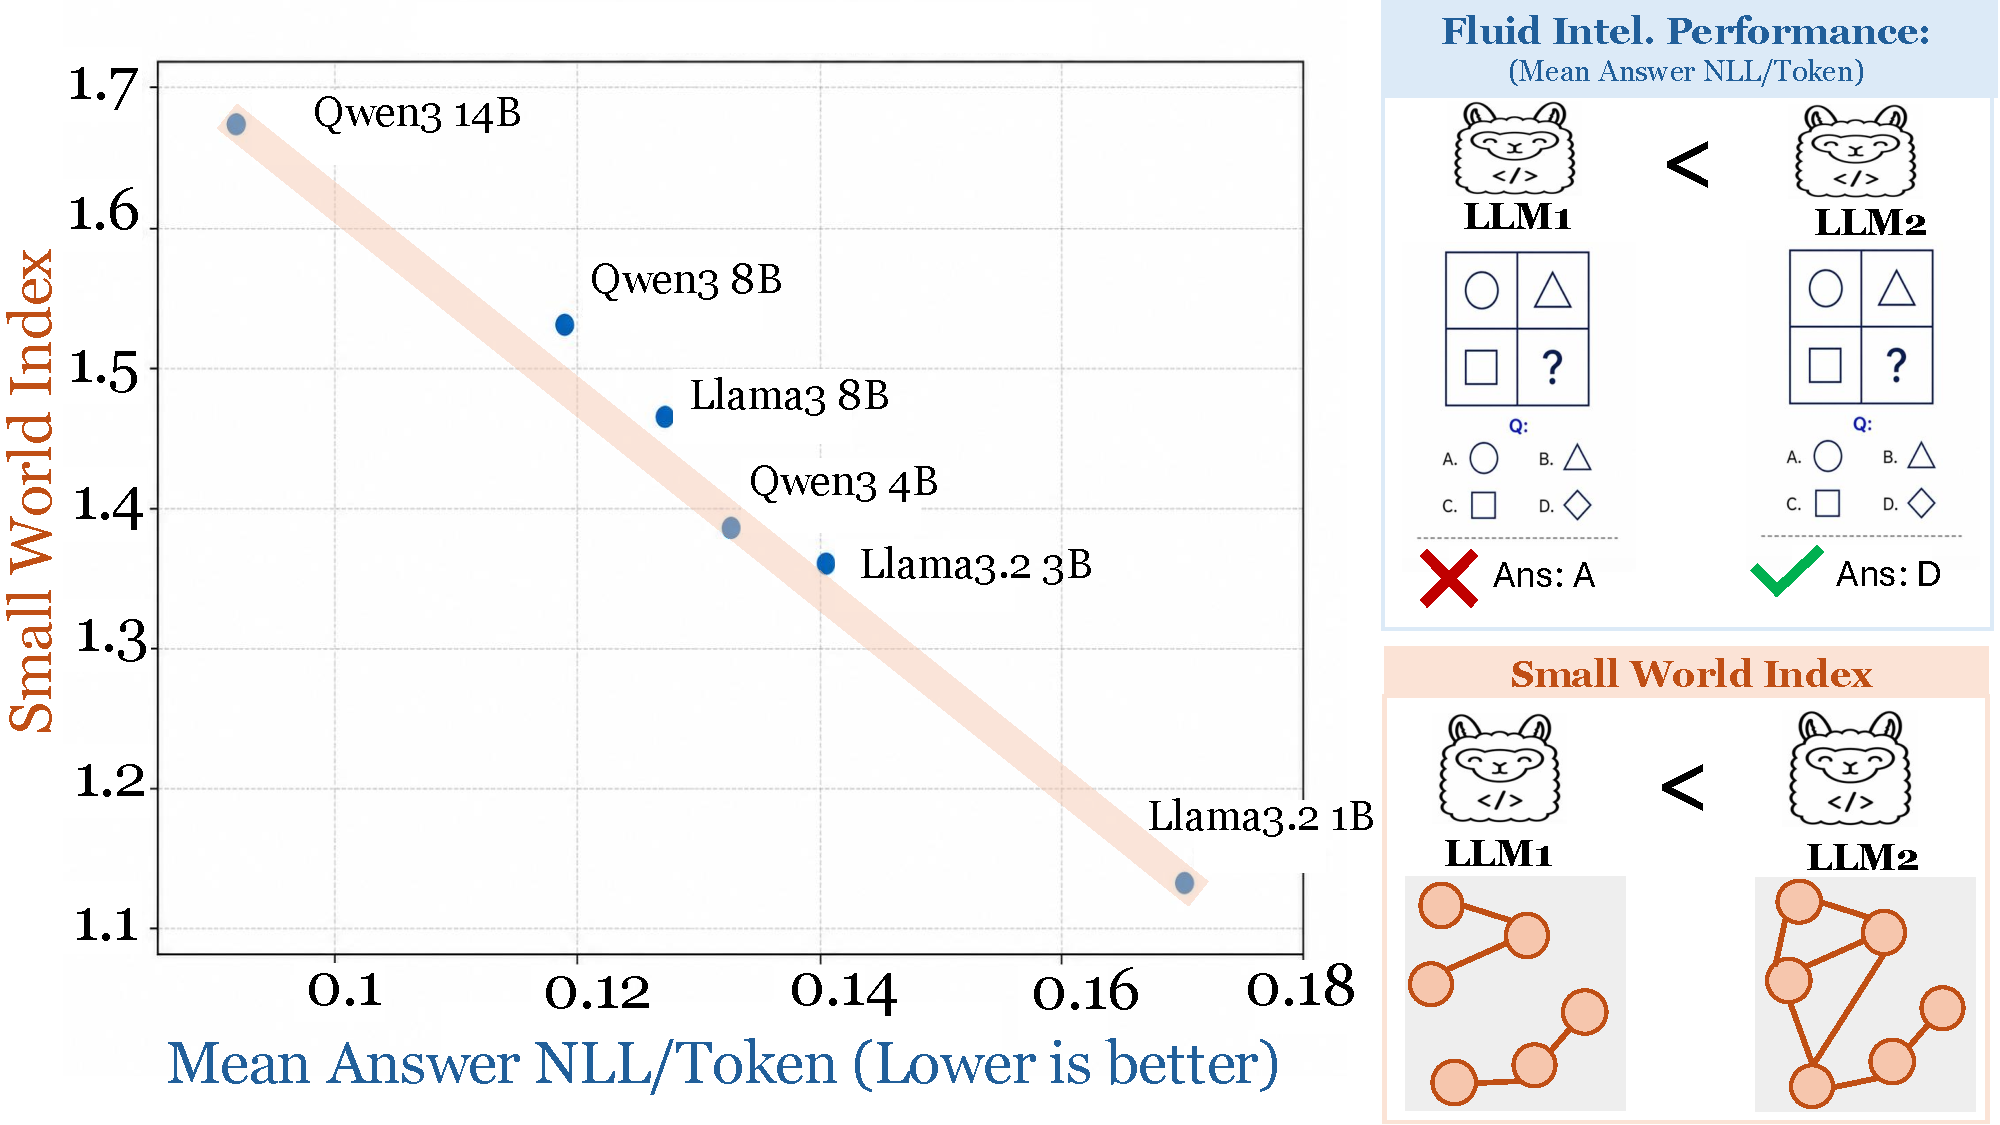
\includegraphics[width=\linewidth]{figure/swi-perf.pdf}
    \caption{\small Across LLMs, a higher small-world index (SWI; y-axis) is consistently associated with better fluid reasoning performance, measured by lower negative log-likelihood (NLL) per answer token on DRE-Bench \cite{yang2025truly} (x-axis).}
    \label{fig:swi-perf}
\end{figure}


In this work, we answer this question by studying the functional organization of LLMs. We focus on attention heads and construct a functional graph in which nodes represent heads and edges are defined by activation similarity. By measuring the small-world organization of this graph, we find that stronger small-world index (SWI) is consistently associated with better fluid reasoning performance across models (\Cref{fig:swi-perf}). 
To validate the importance of this finding, we apply it to LLM pruning, where the goal is to preserve SWI during pruning and evaluate whether the pruned models maintain strong performance. Since SWI is a graph-level measure, we further map it to local model structure by deriving node-level scores based on the two defining properties of small-world networks. Specifically, core scores quantify within-community connectivity related to local clustering, while bridge scores quantify cross-community connectivity related to short communication paths. Building on these local roles, we introduce our pruning method, Small-World Allocation (SWA), which aggregates node-level structural priorities to guide sparsity allocation across layers and attention heads. Experiments show that SWA better preserves both small-world organization and model performance over state-of-the-art pruning baselines.
% Since SWI is a graph-level measure, we derive fine-grained scores to assign small-world organization to individual heads and layers. Specifically, core scores capture within-community connectivity and contribute to local clustering, while bridge scores capture cross-community connectivity and support short communication paths across communities.
% node-level scores based on (!!!at finer granularity, such as heads and layers.\yy{comments not deleted?}) its two defining properties: core scores capture within-community connectivity and contribute to local clustering, while bridge scores capture cross-community connectivity and support short communication paths across communities. 
%yy{briefly say which affects clustering coefficient and which connects to short path length}
% We then introduce Small-World Allocation (SWA), which aggregates these node-level roles into layer- and head-level structural priorities for sparsity allocation. 
% %\yy{need better connection here. see comments in abstract.}
% Using pruning as a validation, we show that SWA better preserves SWI, language modeling quality, and fluid reasoning ability under sparsity. These results suggest that the proposed small-world metrics capture performance-relevant organization in LLMs. 
Our contributions are summarized as follows:
\begin{itemize}
    \item \textbf{Novel Insight:} To our knowledge, we are the first to show that LLMs' attention head activations exhibit a small-world functional organization. We further show that SWI is correlated with performance on fluid intelligence benchmarks and remains consistent across different LLM architectures.

   \item \textbf{Novel Metrics:} We propose small-world metrics that characterize LLM functional organization at multiple levels of granularity. SWI measures graph-level small-world organization, while core and bridge scores assign this organization to individual attention heads by quantifying within-community and cross-community connectivity. We show that these metrics guide effective LLM pruning and consistently correlate with performance on fluid intelligence tasks.
    
    %\yy{what is the goal/usage of our framework? You should say something like we design...to achieve some goal/we propose a novel and general framework to do what..}

    \item \textbf{New Method:} Building on the proposed small-world metrics, we introduce Small-World Allocation (SWA), a hierarchical sparsity allocation method that assigns pruning ratios across layers and heads according to their structural priorities. Experiments show that SWA better preserves small-world organization under pruning and improves language modeling performance by up to $20.01\%$ over state-of-the-art pruning baselines.

    % \yy{a bit vague, don't say structurally important components, you should explicitly say what structural properties you want}
\end{itemize}




%method: 
% exp: preserve more swi
% preserve swi prune better







\section{Preliminaries}
\label{sec:prelim}

\subsection{Notation}

We consider a transformer-based large language model (LLM) with $L$ layers and $H$ attention heads per layer. We denote the set of all attention heads as
$
\mathcal{H} = \{h_{\ell,a} \mid \ell = 1, \ldots, L,\; a = 1, \ldots, H\},
$
where $h_{\ell,a}$ represents the $a$-th head in layer $\ell$. We use $\mathcal{G}=(\mathcal{V},\mathcal{E})$ to denote a graph, where $\mathcal{V}$ is the node set and $\mathcal{E}$ is the edge set. In our functional graphs, nodes correspond to attention heads, i.e., $\mathcal{V}=\mathcal{H}$, and edges are constructed from activation-based similarity between heads.

\subsection{Small-World Organization of Brain Networks}

Small-world organization describes a network topology characterized by high local clustering and efficient global communication \cite{barbey2018network, rosenberg2020functional}. In neuroscience, functional brain networks are often built over anatomical regions of interest (ROIs), with nodes as brain regions and edges as functional connectivity \cite{langer2012functional}. Such organization has been linked to human intelligence: higher Raven's Advanced Progressive Matrices scores \cite{bors2003effect, raven1962advanced} are associated with stronger small-world structure, reflected by higher clustering coefficients and shorter communication path lengths \cite{langer2012functional}.

More generally, given a graph $\mathcal{G}=(\mathcal{V},\mathcal{E})$, let $C(\mathcal{G})$ denote its average clustering coefficient \cite{watts1998collective}, defined as
\begin{equation}
C(\mathcal{G}) =
\frac{1}{|\mathcal{V}|}
\sum_{i\in\mathcal{V}} C_i,
\qquad
C_i =
\frac{2e_i}{d_i(d_i-1)},
\end{equation}
where $d_i$ is the degree of node $i$, $e_i$ is the number of edges among the neighbors of node $i$, and we set $C_i=0$ when $d_i<2$. We let $E(\mathcal{G})$ denote its global efficiency, which captures efficient communication through short paths \cite{latora2001efficient}:
\begin{equation}
E(\mathcal{G}) =
\frac{1}{|\mathcal{V}|(|\mathcal{V}|-1)}
\sum_{\substack{i,j\in\mathcal{V}\\ i\neq j}}
\frac{1}{\operatorname{dist}(i,j)},
\end{equation}
where $\operatorname{dist}(i,j)$ is the shortest-path distance between nodes $i$ and $j$, and disconnected node pairs contribute zero efficiency. To assess small-world organization, $\mathcal{G}$ is compared against degree-preserving randomized graphs generated by edge swaps \cite{hosseini2013influence}. Let $C_{\mathrm{rand}}$ and $E_{\mathrm{rand}}$ denote the average clustering coefficient and global efficiency of these randomized graphs. The small-world index of $\mathcal{G}$ is then defined as
\begin{equation}
\mathrm{SWI}(\mathcal{G}) =
\frac{C(\mathcal{G})}{C_{\mathrm{rand}}}
\cdot
\frac{E(\mathcal{G})}{E_{\mathrm{rand}}}.
\label{eq:swi}
\end{equation}
A larger SWI indicates stronger local clustering and more efficient global communication relative to degree-matched random graphs.


\subsection{SVCCA for Representation Similarity}
\label{sec:svcca_prelim}

We use Singular Vector Canonical Correlation Analysis (SVCCA)~\cite{raghu2017svcca} to measure similarity between vector-valued representations. Given two mean-centered representation matrices
$\mathbf{X}\in\mathbb{R}^{m\times D_x}$ and
$\mathbf{Y}\in\mathbb{R}^{m\times D_y}$ over the same $m$ examples, SVCCA first applies singular value decomposition:
\begin{equation}
\mathbf{X} = \mathbf{U}_X \mathbf{S}_X \mathbf{V}_X^\top,
\qquad
\mathbf{Y} = \mathbf{U}_Y \mathbf{S}_Y \mathbf{V}_Y^\top .
\end{equation}

We retain the top singular directions explaining a high proportion of variance, e.g., $99\%$. Let $p_x$ and $p_y$ be the numbers of retained directions for $\mathbf{X}$ and $\mathbf{Y}$, respectively. The representations are then projected as

\begin{equation}
\mathbf{X}' = \mathbf{X}\mathbf{V}_X^{(p_x)}, 
\qquad
\mathbf{Y}' = \mathbf{Y}\mathbf{V}_Y^{(p_y)} ,
\end{equation}

where $\mathbf{X}'\in\mathbb{R}^{m\times p_x}$ and
$\mathbf{Y}'\in\mathbb{R}^{m\times p_y}$. Here, $\mathbf{V}_X^{(p_x)}$ and $\mathbf{V}_Y^{(p_y)}$
denote the matrices formed by the first $p_x$ and $p_y$ columns of
$\mathbf{V}_X$ and $\mathbf{V}_Y$, respectively.

Canonical Correlation Analysis (CCA)~\cite{thompson2000canonical} then finds projection vectors $\mathbf{w}_x$ and $\mathbf{w}_y$ that maximize the correlation between the projected representations:
$
\rho =
\max_{\mathbf{w}_x, \mathbf{w}_y}
\frac{
\mathbf{w}_x^\top \boldsymbol{\Sigma}_{X'Y'} \mathbf{w}_y
}{
\sqrt{
(\mathbf{w}_x^\top \boldsymbol{\Sigma}_{X'X'} \mathbf{w}_x)
(\mathbf{w}_y^\top \boldsymbol{\Sigma}_{Y'Y'} \mathbf{w}_y)
}
}.
$
Here, $\boldsymbol{\Sigma}_{X'X'}$ and $\boldsymbol{\Sigma}_{Y'Y'}$ denote the covariance matrices of
$\mathbf{X}'$ and $\mathbf{Y}'$, and $\boldsymbol{\Sigma}_{X'Y'}$ denotes their cross-covariance matrix. This produces a set of canonical correlations
$\{\rho_q\}_{q=1}^{r}$, where $r=\min(p_x,p_y)$.
We define the SVCCA similarity as their mean:
\begin{equation}
\mathrm{SVCCA}(\mathbf{X},\mathbf{Y})
=
\frac{1}{r}\sum_{q=1}^{r}\rho_q .
\end{equation}
Higher SVCCA values indicate stronger alignment between representational subspaces.
\section{Key Findings}

\begin{figure}
    \centering
    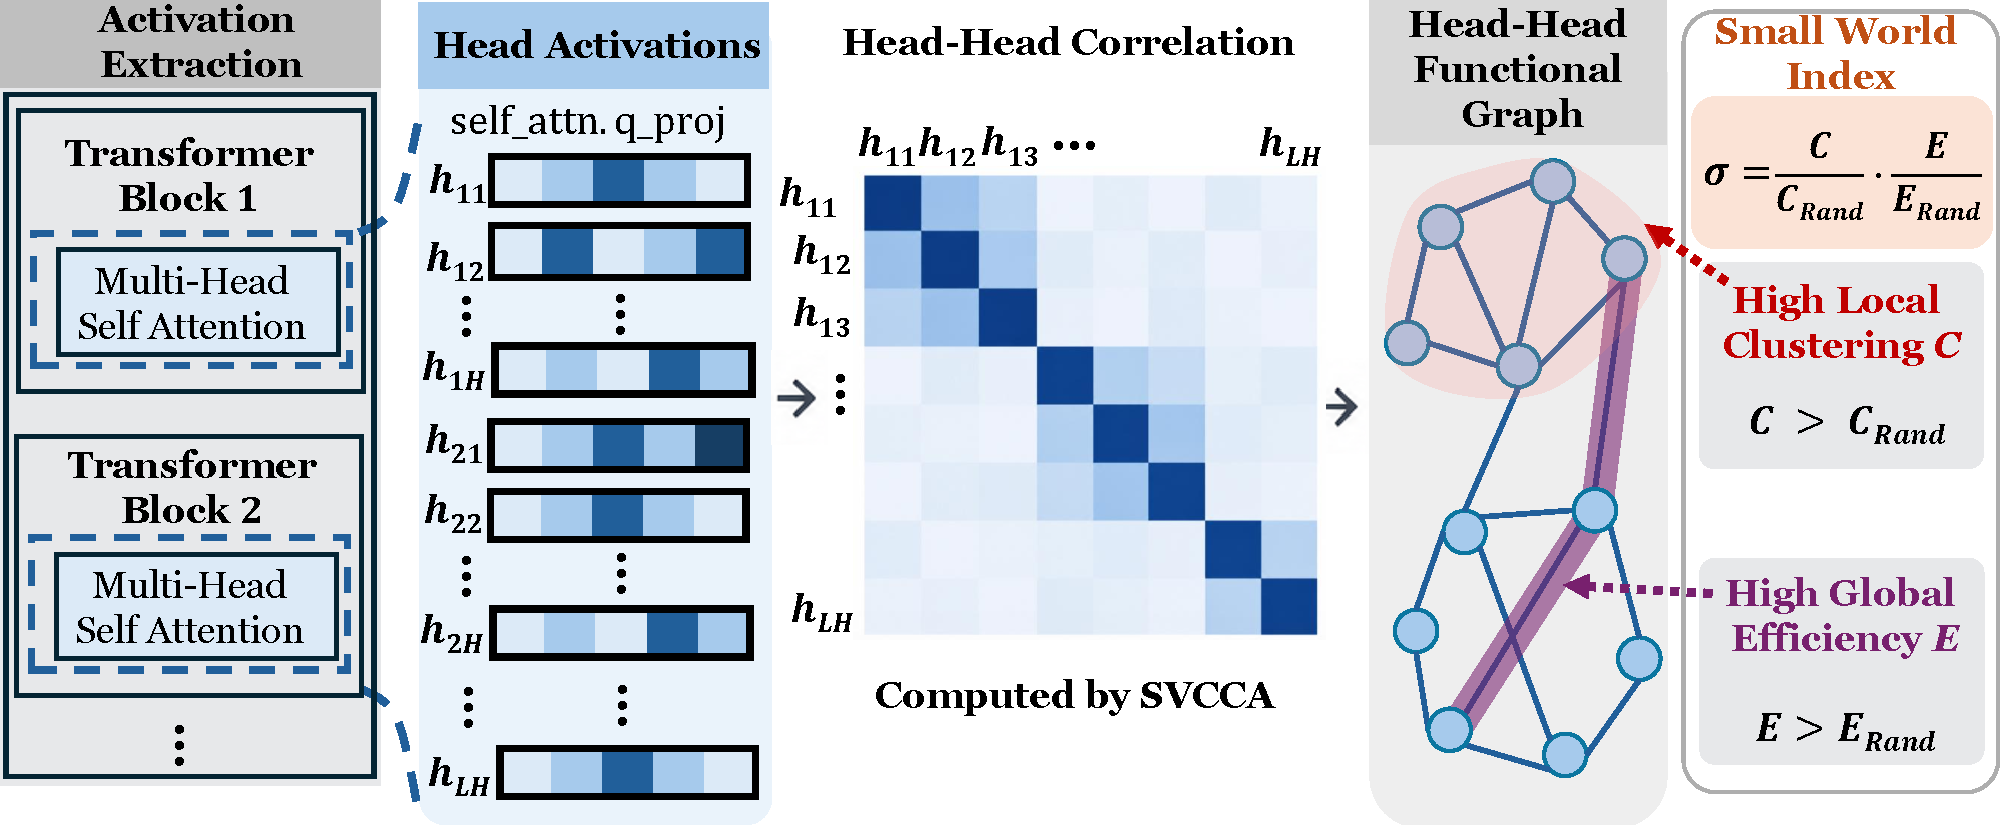
\includegraphics[width=0.85\linewidth]{figure/nips_figure_26_new.pdf}
    \caption{\small We extract activations from attention heads across Transformer layers and compute pairwise similarity (SVCCA) to construct a head-level functional graph. The resulting graph exhibits small-world structure, characterized by high clustering and efficient short-path communication. We show that this structural property correlates with model capability on fluid intelligence benchmarks.}
    \label{fig:process}
\end{figure}

In this section, we present our framework for constructing functional graphs of attention heads and quantifying their small-world organization. We first show how we construct an attention-head functional graph and compute its SWI (\Cref{sec:constructing-head}). Second, we show that SWI is associated with LLM performance on fluid intelligence benchmarks (\Cref{sec:quantify_swi}). The process is shown in~\Cref{fig:process}.



% \subsection{Constructing Functional Graphs of Attention Heads}
% \label{sec:constructing-head}
% \paragraph{Activation collection.}
% We collect attention-head activations on DRE-Bench, a dynamic benchmark for evaluating LLM fluid intelligence through abstract reasoning tasks \cite{yang2025truly}. Its tasks assess attribute-level, spatial, sequential, and conceptual reasoning, and use dynamically generated variants to test whether models can infer latent rules.\yy{the following introduction of the functional graph construction needs major revision. It should be introduced in an organized way: first introduce high level: what are the nodes and what are the edges. then give rationale by linking it to neuroscience. what analogies you are making: brain regions<->attention heads, correlation of activations<->correlation of attention acitivation. then talk a bit in detail, how do you obtain the activations and then how you compute the SVCCA similarity to obtain the edges. Also you need to provide intuition of using SVCCA. You should unlike neuroscience where ROI has scalar activation each time, each attention head produce a vector for each sample, so we need new definition for attention head similarity. This similarity should be invariant to permutation of embedding features and also need to account for the fact that attention heads from different layers may reside in different latent space. Thus, we propose to use SVCCA similarity becasue it satisifies these requirements... Then introduce SVCCA}
% Let an LLM contain $L$ transformer blocks and $H$ attention heads per block, yielding $M=L\times H$ heads in total. We sample $N$ questions from DRE-Bench, denoted as $\{x^{(n)}\}_{n=1}^{N}$. For each question $x^{(n)}$, let $T_n$ denote the number of tokens generated in its answer. We record the query activations of all self-attention heads at each generated answer token, since query activations determine which context tokens each head attends to during generation \cite{elhage2021mathematical}. This yields an activation tensor:
% \[
% \mathbf{A}^{(n)} \in \mathbb{R}^{M \times T_n \times d},
% \]
% where $d$ is the head dimension and $\mathbf{A}^{(n)}_{m,t,:}$ denotes the query activation of head $m$ at the $t$-th generated answer token. For each head and question, we average its token-level activations over the generated answer tokens:
% \[
% \mathbf{z}^{(n)}_m =
% \frac{1}{T_n}\sum_{t=1}^{T_n}\mathbf{A}^{(n)}_{m,t,:},
% \qquad
% \mathbf{z}^{(n)}_m \in \mathbb{R}^{d}.
% \]
% Stacking these vectors over all $N$ questions gives the activation matrix for head $m$:
% \[
% \mathbf{X}_m =
% \left[
% \mathbf{z}^{(1)}_m;
% \mathbf{z}^{(2)}_m;
% \dots;
% \mathbf{z}^{(N)}_m
% \right]
% \in \mathbb{R}^{N\times d}.
% \]
% Each row of $\mathbf{X}_m$ corresponds to the query activation of head $m$ for one DRE-Bench question. We use $\mathbf{X}_m$ to compute activation similarity between pairs of attention heads.






% \paragraph{SVCCA similarity.}
% Given the activation matrices $\{\mathbf{X}_m\}_{m=1}^{M}$, we compute pairwise similarity between attention heads using Singular Vector Canonical Correlation Analysis (SVCCA) \cite{raghu2017svcca}. For each pair of heads $(i,j)$, we first apply singular value decomposition (SVD) to $\mathbf{X}_i$ and $\mathbf{X}_j$ and retain the principal directions that explain a fraction $\tau$ of the variance. 
% %We use $\tau=0.99$ in our experiments. 
% We then apply canonical correlation analysis (CCA)~\cite{thompson2000canonical} to the reduced representations, obtaining canonical correlations $\{\rho_k\}_{k=1}^{r_{ij}}$, where $r_{ij}$ is the number of retained CCA dimensions.

% We define the activation similarity between heads $i$ and $j$ as the average canonical correlation:
% \[
% S_{ij}=\frac{1}{r_{ij}}\sum_{k=1}^{r_{ij}} \rho_k,
% \qquad S_{ii}=1.
% \]
% This yields a symmetric head-similarity matrix $\mathbf{S}\in[0,1]^{M\times M}$, where larger values indicate more similar activation patterns across DRE-Bench questions.
\subsection{Constructing Functional Graphs of Attention Heads}
\label{sec:constructing-head}
% we follow ns to build graph, we 类比 xxxx. we follow the way ns build graph that we xxx. 先算correlation 再算threhold then we show how we create the graph
% have the 3.2 threshold to 3.1, and 3.2 only has finding.
% 

% move svcca to prelim

% sec4 say validate. our idea is that we want to preserve SWI in pruning.

% 4.2 开头：based on the local cores we obtained, we propose. 4.2 add pruing priority scores

% layer include all modules within the block
% assign budge proportional to scores.


We first collect attention-head activations on DRE-Bench~\cite{yang2025truly}, whose tasks assess attribute-level, spatial, sequential, and conceptual reasoning. We follow the standard construction of functional brain networks: anatomical ROIs are treated as nodes, pairwise functional connectivity is estimated from statistical dependencies between their activity time series, and a graph is obtained by thresholding the resulting connectivity matrix. Analogously, we treat attention heads as nodes and estimate pairwise functional connectivity from activation-based similarity between heads. We then threshold the resulting head-similarity matrix to construct an attention-head functional graph.



% In order to build the graph of attention heads, we first collect attention-head activations on DRE-Bench \cite{yang2025truly}, which assess attribute-level, spatial, sequential, and conceptual reasoning. We then define nodes as attention heads and edges as activation-based similarities between heads. This construction is inspired by functional brain networks, where anatomical ROIs are treated as nodes and edges are estimated from statistical dependencies between their activity time series. In brain networks, functional connectivity is often estimated by Pearson correlation between scalar ROI activity time series \cite{biswal1995functional, fox2005human}. Since attention heads produce vector-valued activations, we propose use SVCCA as a multivariate analogue of correlation that measures shared correlated subspaces between heads. Detailed justification of using SVCCA is in \Cref{app:svcca_justification} of the Appendix. \yy{Since you already have a beginning paragraph in Section 3, you do not repeat again. I would suggest delete this paragraph and integrate the information to the following subsections. }

\paragraph{Activation Collection.}
% We collect attention-head activations on DRE-Bench, a dynamic benchmark for evaluating LLM fluid intelligence through abstract reasoning tasks \cite{yang2025truly}. 
% Its tasks assess attribute-level, spatial, sequential, and conceptual reasoning, and use dynamically generated variants to test whether models can infer latent rules.

Let an LLM contain $L$ transformer blocks and $H$ attention heads per block, yielding $M=L\times H$ heads in total. We sample $N$ questions from DRE-Bench \cite{yang2025truly}, denoted as $\{x^{(n)}\}_{n=1}^{N}$. For each question $x^{(n)}$, let $T_n$ denote the number of tokens generated in its answer. We record the query activations of all self-attention heads at each generated answer token.
% , since query activations determine which context tokens each head attends to during generation \cite{elhage2021mathematical}. 
This yields an activation tensor:
$
\mathbf{A}^{(n)} \in \mathbb{R}^{M \times T_n \times d},
$
where $d$ is the head dimension and $\mathbf{A}^{(n)}_{m,t,:}$ denotes the query activation of head $m$ at the $t$-th generated answer token. For each head and question, we average its token-level activations over the generated answer tokens:
$
\mathbf{z}^{(n)}_m =
\frac{1}{T_n}\sum_{t=1}^{T_n}\mathbf{A}^{(n)}_{m,t,:}, \mathbf{z}^{(n)}_m \in \mathbb{R}^{d}.
$

Stacking these vectors over all $N$ questions gives the activation matrix for head $m$:
$
\mathbf{X}_m =
\left[
\mathbf{z}^{(1)}_m;
\mathbf{z}^{(2)}_m;
\dots;
\mathbf{z}^{(N)}_m
\right]
\in \mathbb{R}^{N\times d}.
$
Each row of $\mathbf{X}_m$ corresponds to the query activation of head $m$ for one DRE-Bench question.


\paragraph{SVCCA Similarity.}
In functional brain networks, connectivity is often estimated using Pearson correlation between scalar ROI activity time series~\cite{biswal1995functional, fox2005human}. Attention heads, however, produce vector-valued activations. We therefore use SVCCA as a multivariate analogue of correlation, measuring shared correlated subspaces between heads. Additional justification for using SVCCA is provided in Section~\ref{app:swa_svcca_justification}. To compute pairwise head similarity using SVCCA as defined in~\Cref{sec:svcca_prelim}, we treat the activation matrix $\mathbf{X}_m$ of each head as its representation over DRE-Bench questions. For each pair of heads $(i,j)$, we define
$
S_{ij}=\mathrm{SVCCA}(\mathbf{X}_i,\mathbf{X}_j), S_{ii}=1.
$
This yields a symmetric head-similarity matrix $\mathbf{S}\in[0,1]^{M\times M}$, where larger values indicate more similar activation behavior across DRE-Bench questions.

\paragraph{Graph Construction.}
Following convention to construct brain graphs, we construct the graph of attention heads by thresholding the head-similarity matrix. Let $\mathcal{P}$ denote the set of all unordered pairs of distinct heads. For a target edge density $\delta$, we rank pairs in $\mathcal{P}$ by $S_{ij}$ and retain the top $K_\delta=\lfloor \delta |\mathcal{P}| \rfloor$ pairs as edges. This yields an undirected head--head functional graph
$
\mathcal{G}_\delta=(\mathcal{V},\mathcal{E}_\delta),
$
where $\mathcal{V}=\{1,\ldots,M\}$ is the set of attention heads.


\subsection{Connection of Small-world Index to Fluid Intelligence}
\label{sec:quantify_swi}
We find that \textbf{stronger small-world organization in head-head functional graphs is associated with better fluid reasoning performance} by computing the SWI of $\mathcal{G}_\delta$, following~\Cref{eq:swi}. Specifically, for each model, we compute SWI from the head-head functional graph constructed on DRE-Bench and evaluate performance using the mean per-token negative log-likelihood over the answer tokens (NLL/token), where lower values indicate better performance. As shown in Table~\ref{tab:dre_perf_swi_levels}, models with lower NLL consistently exhibit higher SWI. Qwen3-14B achieves the strongest performance and the highest SWI, while Llama-3.2-1B has the weakest performance and the lowest SWI. The trend remains consistent across models, suggesting that stronger small-world functional organization is associated with better fluid reasoning performance. The setup details are in \Cref{sec:swa_exp_setup}.

\begin{table}[t]
\centering
\small
\setlength{\tabcolsep}{4pt}

\caption{\small Relationship between DRE-Bench performance and small-world organization.
We report the mean per-token negative log-likelihood over the answer tokens (NLL/token; lower is better) and SWI of the head-head functional graph on DRE-Bench Level 1 and Level 2 tasks. Results are averaged over three seeds and reported as mean$_{\pm \text{std}}$. Across models, lower NLL is associated with higher SWI.}

\begin{tabular}{lcccc}
\toprule
\textbf{Model} 
& \multicolumn{2}{c}{\textbf{Level 1}} 
& \multicolumn{2}{c}{\textbf{Level 2}} \\
\cmidrule(lr){2-3} \cmidrule(lr){4-5}
& \textbf{NLL/token} $\downarrow$
& \textbf{SWI} $\uparrow$
& \textbf{NLL/token} $\downarrow$
& \textbf{SWI} $\uparrow$ \\
\midrule
Qwen3 14B 
& 0.0822$_{\scriptstyle \pm 0.01}$ & 1.8160$_{\scriptstyle \pm 0.27}$
& 0.2410$_{\scriptstyle \pm 0.03}$ & 1.7020$_{\scriptstyle \pm 0.12}$ \\
Qwen3 8B 
& 0.0949$_{\scriptstyle \pm 0.01}$ & 1.5850$_{\scriptstyle \pm 0.28}$
& 0.2814$_{\scriptstyle \pm 0.02}$ & 1.6000$_{\scriptstyle \pm 0.07}$\\
Llama3 8B 
& 0.0980$_{\scriptstyle \pm 0.01}$ & 1.3750$_{\scriptstyle \pm 0.19}$
& 0.2993$_{\scriptstyle \pm 0.02}$ & 1.5935$_{\scriptstyle \pm 0.11}$ \\
Qwen3 4B 
& 0.1142$_{\scriptstyle \pm 0.02}$ & 1.2180$_{\scriptstyle \pm 0.26}$
& 0.3397$_{\scriptstyle \pm 0.05}$ & 1.2722$_{\scriptstyle \pm 0.18}$ \\
Llama3.2 3B 
& 0.1377$_{\scriptstyle \pm 0.07}$ & 1.1933$_{\scriptstyle \pm 0.33}$
& 0.3412$_{\scriptstyle \pm 0.10}$ & 1.2100$_{\scriptstyle \pm 0.17}$ \\
Llama3.2 1B 
& 0.1689$_{\scriptstyle \pm 0.20}$ & 0.9188$_{\scriptstyle \pm 0.49}$
& 0.5800$_{\scriptstyle \pm 0.26}$ & 0.9344$_{\scriptstyle \pm 0.18}$ \\
\bottomrule
\end{tabular}
\vspace{-0.5cm}

\label{tab:dre_perf_swi_levels}
\end{table}



% sec4 say validate. our idea is that we want to preserve SWI in pruning.

% 4.2 开头：based on the local cores we obtained, we propose. 4.2 add pruing priority scores

% layer include all modules within the block
% assign budge proportional to scores.
\section{Applying Our Finding to LLM Pruning}
\label{sec:core-bridge}
In this section, we validate the finding in~\Cref{sec:quantify_swi} by testing whether preserving small-world organization helps maintain model performance under pruning. Since SWI is a graph-level metric, while pruning decisions are typically made at finer granularity such as heads and layers, we translate global small-world organization into local measures. Specifically, we define two node-level scores corresponding to the defining properties of small-world organization: local clustering and global communication. We then use these scores to guide sparsity allocation for LLM pruning.


% \yy{Some connecting sentences that transit from the key finding to this section, e.g., From Section 3, we show that maintaining a high SWI is the key to preserve fluid intelligence of LLMs. In this section, we will show how we can apply this finding in LLM pruning. As SWI is a global metric and pruning often takes place at finer granularity, i.e., at the head and layer level. Thus, in this section, we first translate the global SWI into local measures by defining two node-level structural scores that directly capture its defining properties. We then show how we can use these scores to ...}
% In this section, we derive local structural scores from the small-world functional graph, assigning structural roles to individual heads and layers. We then use these scores to guide downstream applications such as pruning.

\subsection{Node-level Small-world Metrics}
Given $\mathcal{G}_\delta$, we define two head-level scores based on the two defining properties of small-world organization. The core score measures within-community connectivity and corresponds to local clustering, while the bridge score measures cross-community connectivity and corresponds to efficient global communication. We apply Louvain community detection~\cite{blondel2008fast} to $\mathcal{G}_\delta$ to obtain communities $\mathcal{C}_\delta=\{C_1,\ldots,C_K\}$, and let $C(i)$ denote the community containing head $i$.
\paragraph{Core Score.}

Let $C(i)$ denote the community containing head $i$, and set $S_{ij}=0$ for non-edge pairs in $\mathcal{G}_\delta$. We define the core score of head $i$ as
$
\mathrm{Core}_i =
\frac{\sum_{j\in C(i)} S_{ij}}
{\sum_{j\in \mathcal{V}} S_{ij} +\varepsilon},
$
where $\varepsilon$ is a small constant that prevents division by zero. A larger $\mathrm{Core}_i$ indicates that a larger fraction of head $i$'s total connection strength lies within its own community, suggesting that the head plays a stronger role in maintaining local community structure.
\paragraph{Bridge Score.}
For head $i$, let
$
s_{i,k}=\sum_{j\in C_k} S_{ij}
\quad\text{and}\quad
s_i=\sum_{j\in\mathcal{V}} S_{ij}.
$
We can then define
$
\mathrm{Bridge}_i
=
1-
\sum_{k=1}^{K}
\left(
\frac{s_{i,k}}{s_i+\varepsilon}
\right)^2.
$
A larger $\mathrm{Bridge}_i$ indicates that head $i$ more strongly links multiple communities \cite{pedersen2017spontaneous}.
Together, core and bridge scores characterize how individual attention heads contribute to the functional graph: core scores capture within-community connectivity, while bridge scores capture cross-community connectivity. We use these scores to guide LLM pruning.


\subsection{Pruning Method Based on Node-Level Small-World Metrics}
\label{sec:pruning}

Based on the local scores we obtained, we propose Small-World Allocation (SWA), a hierarchical sparsity allocation method that uses local small-world scores to guide pruning. The key idea is to preserve components that play important roles in the functional graph. 
SWA defines pruning priority scores at both the head and layer levels: head-level scores determine the pruning ratio for each attention head, while layer-level scores allocate sparsity across Transformer blocks. This two-level design allows SWA to balance local head importance with global layer-wise sparsity allocation.
% SWA therefore defines pruning priority scores at both the head and layer levels: head-level scores determine the pruning ratio for each attention head within a layer, while layer-level scores decide how much sparsity should be assigned to each Transformer block. This two-level design allows SWA to coordinate local head importance with global layer-wise sparsity allocation.

At the head level, we combine core and bridge scores into a pruning priority score. For each head $i$, we first convert its bridge and core scores into percentile ranks over all heads, denoted by $\tilde{B}_i \in [0,1]$ and $\tilde{C}_i \in [0,1]$, where larger values indicate stronger structural roles. We define the priority score as
\begin{equation}
p_i = (1-\tilde{B}_i)(1-\tilde{C}_i).
\end{equation}

A smaller pruning priority score $p_i$ indicates that head $i$ has a strong core or bridge role and should be preserved, while a larger $p_i$ indicates higher pruning priority. At the layer level, we aggregate head-level pruning priority scores within each layer. Let $\mathcal{H}_\ell$ denote the set of heads in layer $\ell$
\begin{equation}
p_\ell =
\frac{1}{|\mathcal{H}_\ell|}
\sum_{i\in \mathcal{H}_\ell}
p_i .
\end{equation}

A smaller score $p_\ell$ indicates that layer $\ell$ contains more structurally important heads and should receive a lower sparsity budget, while a larger $p_\ell$ indicates higher layer-level pruning priority.

SWA assigns pruning budgets in proportion to the priority scores through a hierarchical allocation procedure. Layer-level scores first determine the sparsity budget for each Transformer block, including all modules within the block; head-level scores then distribute the attention sparsity across individual heads. Following~\cite{hu2025eigenspectrum}, we normalize the scores, convert them into relative pruning ratios, and rescale the ratios so that the overall sparsity matches the target global sparsity.

\section{Experiments}
\begin{table}[t]
\centering
\small
\setlength{\tabcolsep}{3.0pt}
\caption{\small 
We report the small-world index (SWI $\uparrow$) of head-head functional graphs after applying SparseGPT and its variants at sparsity 0.5. 
 SWA (Head) and SWA (Layer) denote head-only and layer-only allocation strategies, respectively. 
\textbf{Higher SWI indicates better preservation} of small-world functional organization under pruning. Results are averaged over three seeds and reported as mean$_{\pm \text{std}}$.
The best result for each model is \colorbox{gray!15}{\textbf{bolded}}.
}
\resizebox{0.8\linewidth}{!}{

\begin{tabular}{lcccccc}
\toprule
\textbf{Model} 
& \textbf{SparseGPT} 
& \textbf{+ FARMS} 
& \textbf{+ ATP} 
& \textbf{+ SWA (Head)} 
& \textbf{+ SWA (Layer)} 
& \textbf{+ SWA} \\
\midrule
Qwen3 14B     & 0.1748$_{\scriptstyle \pm 0.06}$ & 0.1732$_{\scriptstyle \pm 0.06}$ & 0.1631$_{\scriptstyle \pm 0.09}$ & 0.1710$_{\scriptstyle \pm 0.09}$ & 0.1832$_{\scriptstyle \pm 0.08}$ & \colorbox{gray!15}{\textbf{0.1982}$_{\scriptstyle \pm 0.07}$} \\
Qwen3 8B      & 0.1470$_{\scriptstyle \pm 0.05}$ & 0.1560$_{\scriptstyle \pm 0.06}$ & 0.1418$_{\scriptstyle \pm 0.06}$ & 0.1545$_{\scriptstyle \pm 0.07}$ & 0.1606$_{\scriptstyle \pm 0.04}$ & \colorbox{gray!15}{\textbf{0.1775}$_{\scriptstyle \pm 0.05}$} \\
Qwen3 4B      & 0.1148$_{\scriptstyle \pm 0.10}$ & 0.1200$_{\scriptstyle \pm 0.09}$ & 0.1198$_{\scriptstyle \pm 0.05}$ & 0.1330$_{\scriptstyle \pm 0.08}$ & 0.1327$_{\scriptstyle \pm 0.05}$ & \colorbox{gray!15}{\textbf{0.1431}$_{\scriptstyle \pm 0.06}$} \\
\midrule
Llama3 8B    & 0.1285$_{\scriptstyle \pm 0.05}$ & 0.1420$_{\scriptstyle \pm 0.07}$ & 0.1227$_{\scriptstyle \pm 0.08}$ & 0.1341$_{\scriptstyle \pm 0.07}$ & 0.1420$_{\scriptstyle \pm 0.08}$ & \colorbox{gray!15}{\textbf{0.1599}$_{\scriptstyle \pm 0.06}$} \\
Llama3.2 3B  & 0.0772$_{\scriptstyle \pm 0.05}$ & 0.0880$_{\scriptstyle \pm 0.02}$ & 0.0898$_{\scriptstyle \pm 0.04}$ & 0.0877$_{\scriptstyle \pm 0.06}$ & 0.1005$_{\scriptstyle \pm 0.04}$ & \colorbox{gray!15}{\textbf{0.1126}$_{\scriptstyle \pm 0.04}$} \\
Llama3.2 1B  & 0.0558$_{\scriptstyle \pm 0.04}$ & 0.0520$_{\scriptstyle \pm 0.05}$ & 0.0524$_{\scriptstyle \pm 0.05}$ & 0.0559$_{\scriptstyle \pm 0.03}$ & 0.0661$_{\scriptstyle \pm 0.03}$ & \colorbox{gray!15}{\textbf{0.0700}$_{\scriptstyle \pm 0.04}$} \\
\bottomrule
\end{tabular}
}
\label{tab:swi_pruning_preservation}

\end{table}
\begin{table*}[t]
\centering
\scriptsize
\setlength{\tabcolsep}{2.0pt}
\caption{\small  Comparison of \textbf{WikiText Perplexity ($\downarrow$)}. We evaluate Base pruning methods (Wanda and SparseGPT) and their variants augmented with FARMS, ATP, and SWA at sparsity 0.5/0.7. Results are averaged over three seeds and reported as mean$_{\pm \text{std}}$. The best result in each setting is \colorbox{gray!15}{\textbf{bolded}}. SWA reduces perplexity and achieves the best values across all the models and sparsity levels.}
\begin{tabular}{ccc|llll|llll}
\toprule
\multirow{2}{*}{\textbf{Model}} & \multirow{2}{*}{\textbf{Size}} & \multirow{2}{*}{\textbf{Sparsity}} & \multicolumn{4}{c|}{\textbf{Wanda}} & \multicolumn{4}{c}{\textbf{SparseGPT}} \\
 &  &  & Base & + FARMS & + ATP & \textbf{+ SWA} & Base & + FARMS & + ATP & \textbf{+ SWA} \\
\midrule
\multirow{4}{*}{\shortstack{Llama 3.2}} & \multirow{2}{*}{1B} & 0.5 & 36.25$_{\scriptstyle \pm 0.18}$ & 33.90$_{\scriptstyle \pm 0.02}$ & 24.95$_{\scriptstyle \pm 0.04}$ & \cellcolor{gray!15}\textbf{22.42$_{\scriptstyle \pm 0.05}$} & 21.54$_{\scriptstyle \pm 0.29}$ & 21.14$_{\scriptstyle \pm 0.56}$ & 20.56$_{\scriptstyle \pm 0.34}$ & \cellcolor{gray!15}\textbf{20.47$_{\scriptstyle \pm 0.15}$} \\
 &  & 0.7 & 415.60$_{\scriptstyle \pm 32.1}$& 380.20$_{\scriptstyle \pm 20.1}$& 264.10$_{\scriptstyle \pm 21.7}$& \cellcolor{gray!15}\textbf{256.67$_{\scriptstyle \pm 18.00}$} & 157.20$_{\scriptstyle \pm 3.2}$& 136.80$_{\scriptstyle \pm 5.3}$& 106.60$_{\scriptstyle \pm 3.2}$& \cellcolor{gray!15}\textbf{105.00$_{\scriptstyle \pm 3.6}$} \\
 & \multirow{2}{*}{3B} & 0.5 & 19.71$_{\scriptstyle \pm 0.02}$ & 16.45$_{\scriptstyle \pm 0.09}$ & 14.42$_{\scriptstyle \pm 0.02}$ & \cellcolor{gray!15}\textbf{13.32$_{\scriptstyle \pm 0.12}$} & 23.98$_{\scriptstyle \pm 2.15}$ & 15.92$_{\scriptstyle \pm 1.85}$ & 13.53$_{\scriptstyle \pm 0.08}$ & \cellcolor{gray!15}\textbf{11.27$_{\scriptstyle \pm 0.98}$} \\
 &  & 0.7 & 177.80$_{\scriptstyle \pm 5.6}$ & 132.6$_{\scriptstyle \pm 5.3}$ & 125.1$_{\scriptstyle \pm 0.8}$ & \cellcolor{gray!15}\textbf{120.65$_{\scriptstyle \pm 2.31}$} & 70.70$_{\scriptstyle \pm 5.07}$ & 67.67$_{\scriptstyle \pm 2.93}$ & 51.51$_{\scriptstyle \pm 3.83}$ & \cellcolor{gray!15}\textbf{49.56$_{\scriptstyle \pm 0.92}$} \\
\multirow{2}{*}{\shortstack{Llama 3}} & \multirow{2}{*}{8B} & 0.5 & 11.86$_{\scriptstyle \pm 0.02}$ & 11.12$_{\scriptstyle \pm 0.03}$ & 11.50$_{\scriptstyle \pm 0.05}$ & \cellcolor{gray!15}\textbf{10.14$_{\scriptstyle \pm 0.03}$} & 11.69$_{\scriptstyle \pm 0.13}$ & 11.02$_{\scriptstyle \pm 0.87}$ & 10.72$_{\scriptstyle \pm 0.15}$ & \cellcolor{gray!15}\textbf{10.15$_{\scriptstyle \pm 0.08}$} \\
 &  & 0.7 & 140.50$_{\scriptstyle \pm 2.6}$ & 90.02$_{\scriptstyle \pm 3.00}$ & 85.93$_{\scriptstyle \pm 0.82}$ & \cellcolor{gray!15}\textbf{84.98$_{\scriptstyle \pm 0.20}$} & 55.94$_{\scriptstyle \pm 3.23}$ & 52.55$_{\scriptstyle \pm 1.98}$ & 40.40$_{\scriptstyle \pm 1.94}$ & \cellcolor{gray!15}\textbf{38.75$_{\scriptstyle \pm 1.29}$} \\
\midrule
\multirow{6}{*}{\shortstack{Qwen 3}} & \multirow{2}{*}{4B} & 0.5 & 21.91$_{\scriptstyle \pm 2.08}$ & 19.69$_{\scriptstyle \pm 0.16}$ & 18.88$_{\scriptstyle \pm 0.03}$ & \cellcolor{gray!15}\textbf{17.86$_{\scriptstyle \pm 0.49}$} & 20.52$_{\scriptstyle \pm 0.43}$ & 19.58$_{\scriptstyle \pm 0.41}$ & 20.44$_{\scriptstyle \pm 0.45}$ & \cellcolor{gray!15}\textbf{19.30$_{\scriptstyle \pm 0.77}$} \\
 &  & 0.7 & 101.80$_{\scriptstyle \pm 3.9}$ & 90.49$_{\scriptstyle \pm 4.84}$ & 64.78$_{\scriptstyle \pm 1.21}$ & \cellcolor{gray!15}\textbf{63.65$_{\scriptstyle \pm 0.27}$} & 50.93$_{\scriptstyle \pm 1.62}$ & 44.30$_{\scriptstyle \pm 2.26}$ & 46.45$_{\scriptstyle \pm 0.91}$ & \cellcolor{gray!15}\textbf{40.24$_{\scriptstyle \pm 0.38}$} \\
 & \multirow{2}{*}{8B} & 0.5 & 14.90$_{\scriptstyle \pm 0.48}$ & 13.20$_{\scriptstyle \pm 0.03}$ & 12.91$_{\scriptstyle \pm 0.06}$ & \cellcolor{gray!15}\textbf{11.90$_{\scriptstyle \pm 0.09}$} & 15.09$_{\scriptstyle \pm 0.07}$ & 12.61$_{\scriptstyle \pm 0.12}$ & 13.08$_{\scriptstyle \pm 0.09}$ & \cellcolor{gray!15}\textbf{12.10$_{\scriptstyle \pm 0.14}$} \\
 &  & 0.7 & 71.10$_{\scriptstyle \pm 1.86}$ & 65.46$_{\scriptstyle \pm 1.51}$ & 57.31$_{\scriptstyle \pm 1.28}$ & \cellcolor{gray!15}\textbf{54.05$_{\scriptstyle \pm 1.62}$} & 30.05$_{\scriptstyle \pm 0.66}$ & 25.13$_{\scriptstyle \pm 1.07}$ & 28.93$_{\scriptstyle \pm 0.43}$ & \cellcolor{gray!15}\textbf{20.10$_{\scriptstyle \pm 0.14}$} \\
 & \multirow{2}{*}{14B} & 0.5 & 11.43$_{\scriptstyle \pm 0.04}$ & 11.38$_{\scriptstyle \pm 0.04}$ & 10.79$_{\scriptstyle \pm 0.04}$ & \cellcolor{gray!15}\textbf{10.02$_{\scriptstyle \pm 0.03}$} & 11.51$_{\scriptstyle \pm 0.05}$ & 11.36$_{\scriptstyle \pm 0.02}$ & 10.92$_{\scriptstyle \pm 0.10}$ & \cellcolor{gray!15}\textbf{9.95$_{\scriptstyle \pm 0.13}$} \\
 &  & 0.7 & 37.04$_{\scriptstyle \pm 0.52}$ & 35.62$_{\scriptstyle \pm 0.27}$ & 34.29$_{\scriptstyle \pm 0.65}$ & \cellcolor{gray!15}\textbf{33.71$_{\scriptstyle \pm 0.45}$} & 20.82$_{\scriptstyle \pm 0.35}$ & 20.18$_{\scriptstyle \pm 0.16}$ & 20.37$_{\scriptstyle \pm 0.23}$ & \cellcolor{gray!15}\textbf{18.90$_{\scriptstyle \pm 0.28}$} \\
\bottomrule
\end{tabular}
\label{tab:ppl}
\vspace{-0.5cm}

\end{table*}

\begin{table*}[t]
\centering
\scriptsize
\setlength{\tabcolsep}{2.0pt}
\caption{\small Comparison of Zero-shot Accuracy  ($\uparrow$). We evaluate Base pruning methods (Wanda and SparseGPT) and their variants augmented with FARMS, ATP, and SWA at sparsity 0.5/0.7. Results are averaged over three seeds and reported as mean$_{\pm \text{std}}$. The best result in each setting is \colorbox{gray!15}{\textbf{bolded}}. SWA improves zero-shot accuracy and achieves the strongest performance over all the models and sparsity levels.}
\begin{tabular}{ccc|llll|llll}
\toprule
\multirow{2}{*}{\textbf{Model}} & \multirow{2}{*}{\textbf{Size}} & \multirow{2}{*}{\textbf{Sparsity}} & \multicolumn{4}{c|}{\textbf{Wanda}} & \multicolumn{4}{c}{\textbf{SparseGPT}} \\
 &  &  & Base & + FARMS & + ATP & \textbf{+ SWA} & Base & + FARMS & + ATP & \textbf{+ SWA} \\
\midrule
\multirow{4}{*}{\shortstack{Llama 3.2}} & \multirow{2}{*}{1B} & 0.5 & 34.91$_{\scriptstyle \pm 3.67}$ & 35.21$_{\scriptstyle \pm 2.28}$ & 37.16$_{\scriptstyle \pm 0.82}$ & \cellcolor{gray!15}\textbf{38.89$_{\scriptstyle \pm 1.03}$} & 39.57$_{\scriptstyle \pm 2.67}$ & 40.33$_{\scriptstyle \pm 2.41}$ & 41.26$_{\scriptstyle \pm 0.23}$ & \cellcolor{gray!15}\textbf{42.85$_{\scriptstyle \pm 1.75}$} \\
 &  & 0.7 & 25.86$_{\scriptstyle \pm 3.62}$ & 27.29$_{\scriptstyle \pm 4.75}$ & 29.86$_{\scriptstyle \pm 4.65}$ & \cellcolor{gray!15}\textbf{31.11$_{\scriptstyle \pm 4.81}$} & 30.85$_{\scriptstyle \pm 4.67}$ & 29.38$_{\scriptstyle \pm 1.33}$ & 35.29$_{\scriptstyle \pm 0.22}$ & \cellcolor{gray!15}\textbf{35.56$_{\scriptstyle \pm 0.34}$} \\
 & \multirow{2}{*}{3B} & 0.5 & 40.53$_{\scriptstyle \pm 1.41}$ & 42.71$_{\scriptstyle \pm 1.22}$ & 44.57$_{\scriptstyle \pm 1.39}$ & \cellcolor{gray!15}\textbf{44.72$_{\scriptstyle \pm 1.87}$} & 45.50$_{\scriptstyle \pm 0.36}$ & 46.67$_{\scriptstyle \pm 0.50}$ & 46.05$_{\scriptstyle \pm 1.41}$ & \cellcolor{gray!15}\textbf{48.49$_{\scriptstyle \pm 0.31}$} \\
 &  & 0.7 & 40.16$_{\scriptstyle \pm 2.41}$ & 41.50$_{\scriptstyle \pm 1.63}$ & 40.91$_{\scriptstyle \pm 4.74}$ & \cellcolor{gray!15}\textbf{43.04$_{\scriptstyle \pm 0.87}$} & 40.42$_{\scriptstyle \pm 1.16}$ & 42.25$_{\scriptstyle \pm 0.85}$ & 41.69$_{\scriptstyle \pm 4.46}$ & \cellcolor{gray!15}\textbf{43.57$_{\scriptstyle \pm 1.11}$} \\
\multirow{2}{*}{\shortstack{Llama 3}} & \multirow{2}{*}{8B} & 0.5 & 52.12$_{\scriptstyle \pm 1.25}$ & 53.49$_{\scriptstyle \pm 2.17}$ & 52.43$_{\scriptstyle \pm 1.32}$ & \cellcolor{gray!15}\textbf{55.22$_{\scriptstyle \pm 1.52}$} & 48.53$_{\scriptstyle \pm 2.24}$ & 50.28$_{\scriptstyle \pm 1.30}$ & 53.48$_{\scriptstyle \pm 0.61}$ & \cellcolor{gray!15}\textbf{54.56$_{\scriptstyle \pm 0.85}$} \\
 &  & 0.7 & 27.57$_{\scriptstyle \pm 0.07}$ & 27.14$_{\scriptstyle \pm 1.84}$ & 35.90$_{\scriptstyle \pm 0.74}$ & \cellcolor{gray!15}\textbf{36.75$_{\scriptstyle \pm 0.72}$} & 37.26$_{\scriptstyle \pm 5.39}$ & 38.38$_{\scriptstyle \pm 0.90}$ & 42.33$_{\scriptstyle \pm 2.86}$ & \cellcolor{gray!15}\textbf{43.32$_{\scriptstyle \pm 1.56}$} \\
\midrule
\multirow{6}{*}{\shortstack{Qwen 3}} & \multirow{2}{*}{4B} & 0.5 & 45.69$_{\scriptstyle \pm 3.35}$ & 46.33$_{\scriptstyle \pm 2.49}$ & 47.45$_{\scriptstyle \pm 0.39}$ & \cellcolor{gray!15}\textbf{47.85$_{\scriptstyle \pm 0.42}$} & 43.75$_{\scriptstyle \pm 1.25}$ & 47.28$_{\scriptstyle \pm 1.04}$ & 46.95$_{\scriptstyle \pm 4.51}$ & \cellcolor{gray!15}\textbf{48.00$_{\scriptstyle \pm 1.23}$} \\
 &  & 0.7 & 35.86$_{\scriptstyle \pm 0.06}$ & 36.60$_{\scriptstyle \pm 1.64}$ & 36.98$_{\scriptstyle \pm 0.48}$ & \cellcolor{gray!15}\textbf{38.00$_{\scriptstyle \pm 0.51}$} & 41.21$_{\scriptstyle \pm 4.51}$ & 42.50$_{\scriptstyle \pm 0.89}$ & 42.00$_{\scriptstyle \pm 4.02}$ & \cellcolor{gray!15}\textbf{43.02$_{\scriptstyle \pm 1.23}$} \\
 & \multirow{2}{*}{8B} & 0.5 & 52.50$_{\scriptstyle \pm 0.89}$ & 53.28$_{\scriptstyle \pm 0.77}$ & 55.38$_{\scriptstyle \pm 0.19}$ & \cellcolor{gray!15}\textbf{56.12$_{\scriptstyle \pm 0.24}$} & 53.04$_{\scriptstyle \pm 3.22}$ & 54.11$_{\scriptstyle \pm 2.70}$ & 55.64$_{\scriptstyle \pm 0.86}$ & \cellcolor{gray!15}\textbf{55.67$_{\scriptstyle \pm 0.66}$} \\
 &  & 0.7 & 38.95$_{\scriptstyle \pm 2.04}$ & 39.57$_{\scriptstyle \pm 0.53}$ & 39.64$_{\scriptstyle \pm 0.53}$ & \cellcolor{gray!15}\textbf{41.66$_{\scriptstyle \pm 0.88}$} & 42.24$_{\scriptstyle \pm 0.52}$ & 42.91$_{\scriptstyle \pm 1.72}$ & 43.48$_{\scriptstyle \pm 0.74}$ & \cellcolor{gray!15}\textbf{44.87$_{\scriptstyle \pm 0.67}$} \\
 & \multirow{2}{*}{14B} & 0.5 & 57.05$_{\scriptstyle \pm 0.44}$ & 57.31$_{\scriptstyle \pm 0.22}$ & 57.86$_{\scriptstyle \pm 1.15}$ & \cellcolor{gray!15}\textbf{58.02$_{\scriptstyle \pm 0.45}$} & 57.12$_{\scriptstyle \pm 0.39}$ & 57.62$_{\scriptstyle \pm 4.73}$ & 57.38$_{\scriptstyle \pm 0.15}$ & \cellcolor{gray!15}\textbf{58.10$_{\scriptstyle \pm 0.34}$} \\
 &  & 0.7 & 43.91$_{\scriptstyle \pm 3.11}$ & 44.69$_{\scriptstyle \pm 2.42}$ & 45.41$_{\scriptstyle \pm 0.93}$ & \cellcolor{gray!15}\textbf{46.44$_{\scriptstyle \pm 2.86}$} & 48.43$_{\scriptstyle \pm 2.22}$ & 49.11$_{\scriptstyle \pm 1.80}$ & 48.97$_{\scriptstyle \pm 2.01}$ & \cellcolor{gray!15}\textbf{49.93$_{\scriptstyle \pm 2.22}$} \\
\bottomrule
\end{tabular}
\label{tab:zero}
\end{table*}

\begin{table*}[t]
\centering
\scriptsize
\setlength{\tabcolsep}{6pt}

\caption{\small ARAOC task mismatch rate at sparsity 0.5. We report mismatch rate (Not M $\downarrow$) across six tasks. Results are averaged over five runs and reported as mean$_{\pm \text{std}}$. The best result in each setting is \colorbox{gray!15}{\textbf{bolded}}.}

\begin{tabular}{l|cccccc}
\toprule
\textbf{Method} 
& \textbf{Move} 
& \textbf{Change Color} 
& \textbf{Copy} 
& \textbf{Mirror} 
& \textbf{Fill Internal} 
& \textbf{Scale} \\
\midrule

Qwen3 8B (Non-Pruned) 
& 36.00$_{\scriptstyle \pm 4.11}$
& 23.14$_{\scriptstyle \pm 4.61}$
& 12.18$_{\scriptstyle \pm 4.12}$
& 84.66$_{\scriptstyle \pm 3.20}$
& 6.07$_{\scriptstyle \pm 1.99}$
& 83.33$_{\scriptstyle \pm 5.87}$ \\
\midrule

SparseGPT 
& 44.21$_{\scriptstyle \pm 9.20}$
& 48.87$_{\scriptstyle \pm 10.40}$
& 60.99$_{\scriptstyle \pm 10.67}$
& 94.76$_{\scriptstyle \pm 9.21}$
& 34.25$_{\scriptstyle \pm 4.67}$
& 88.91$_{\scriptstyle \pm 8.03}$ \\

SparseGPT + FARMS 
& 46.22$_{\scriptstyle \pm 8.21}$
& 50.77$_{\scriptstyle \pm 15.85}$
& 56.60$_{\scriptstyle \pm 12.80}$
& 96.66$_{\scriptstyle \pm 10.76}$
& 33.11$_{\scriptstyle \pm 5.11}$
& 88.06$_{\scriptstyle \pm 8.95}$ \\

SparseGPT + ATP 
& 43.08$_{\scriptstyle \pm 9.01}$
& 47.78$_{\scriptstyle \pm 8.66}$
& 56.77$_{\scriptstyle \pm 12.48}$
& 93.55$_{\scriptstyle \pm 9.63}$
& 32.65$_{\scriptstyle \pm 5.81}$
& 89.48$_{\scriptstyle \pm 7.47}$ \\

SparseGPT + \textbf{SWA} 
& \cellcolor{gray!15}\textbf{41.41$_{\scriptstyle \pm 9.39}$}
& \cellcolor{gray!15}\textbf{47.07$_{\scriptstyle \pm 9.68}$}
& \cellcolor{gray!15}\textbf{56.11$_{\scriptstyle \pm 11.62}$}
& \cellcolor{gray!15}\textbf{91.28$_{\scriptstyle \pm 8.99}$}
& \cellcolor{gray!15}\textbf{30.69$_{\scriptstyle \pm 4.17}$}
& \cellcolor{gray!15}\textbf{86.20$_{\scriptstyle \pm 8.17}$} \\

\bottomrule
\end{tabular}
\vspace{-0.5cm}

\label{tab:araoc_split}
\end{table*}
\begin{table}[t]
\centering
\small
\setlength{\tabcolsep}{6pt}
\caption{ \small Ablation study on hierarchical structural deletion. We report the absolute WikiText perplexity (PPL ↓) of SWA and the PPL increase of each ablated variant relative to SWA under sparsity 0.5 and 0.7. SWA(Layer) uses only layer-level scores, and SWA(Head) uses only head-level scores.}
\label{tab:ablation_hier}
\begin{tabular}{lcccc}
\toprule
\multirow{2}{*}{\textbf{Variant}} 
& \multicolumn{2}{c}{\textbf{SparseGPT}} 
& \multicolumn{2}{c}{\textbf{Wanda}} \\
\cmidrule(lr){2-3} \cmidrule(lr){4-5}
& \textbf{0.5} & \textbf{0.7} 
& \textbf{0.5} & \textbf{0.7} \\
\midrule
\textbf{SWA} 
& \textbf{11.27} & \textbf{49.56} 
& \textbf{13.32} & \textbf{120.65} \\
SWA(Layer) 
& $+3.31$ & $+11.37$ 
& $+0.05$ & $+6.96$ \\
SWA(Head) 
& $+3.63$ & $+19.56$ 
& $+0.24$ & $+46.51$ \\
\bottomrule
\end{tabular}
\vspace{-0.5cm}
\end{table}



We conduct experiments to evaluate whether small-world functional organization is associated with LLM reasoning ability, and whether scores derived from this organization can preserve small-world structure during pruning. Our evaluation is guided by three research questions: \textbf{RQ1.} Does SWA preserve small-world functional organization when used to guide pruning? \textbf{RQ2.} Does pruning with SWA better maintain model performance under sparsity than existing pruning baselines? \textbf{RQ3.} Does pruning with SWA preserve intelligence-related reasoning ability on held-out reasoning benchmarks?

\vspace{-0.2cm}
\subsection{Experimental Setup}
\label{sec:swa_exp_setup}

First, we describe the setup used to collect activations, construct attention-head functional graphs, and compute SWI. Second, we describe the pruning setup used to evaluate whether SWA preserves performance and reasoning ability under sparsity. Details are provided in Section~\ref{app:swa_expdetails}.


\paragraph{Setup for SWI analysis.}
We first evaluate the relationship between SWI and reasoning performance using six open-source LLMs: Qwen3-4B, Qwen3-8B, Qwen3-14B, Llama-3.2-1B, Llama-3.2-3B, and Meta-Llama-3-8B \cite{yang2025qwen3, grattafiori2024llama}. We collect attention-head activations on DRE-Bench \cite{yang2025truly}, using Level 1 and Level 2 questions as calibration inputs for constructing attention-head functional graphs. We exclude Level 3 and Level 4 because current open-source models often fail on these harder tasks, making their generated answers unreliable for activation-based analysis. We evaluate DRE-Bench performance by computing the mean per-token negative log-likelihood over the answer tokens (mean answer NLL/token; lower is better) and compare it with each model's SWI.

\paragraph{Setup for pruning evaluation.}
For pruning experiments, we use the same six LLMs and apply SWA to SparseGPT \cite{frantar2023sparsegpt} and Wanda \cite{sun2023simple}. We compare against uniform sparsity and layer-wise allocation baselines, including FARMS \cite{hu2025eigenspectrum} and ATP \cite{huang2025determining}. We evaluate pruned models using WikiText perplexity \cite{merity2016pointer} and average zero-shot accuracy over BoolQ \cite{clark2019boolq}, RTE \cite{wang2018glue}, HellaSwag \cite{zellers2019hellaswag}, WinoGrande \cite{sakaguchi2021winogrande}, ARC-Easy, ARC-Challenge \cite{clark2018think}, and OpenBookQA \cite{mihaylov2018can} datasets.


\subsection{Effectiveness of Preserving SWI}

To answer \textbf{RQ1}, we evaluate whether SWA preserves small-world functional organization during pruning. For each of the six models, we apply SparseGPT at a sparsity level of $0.5$ and compare it with variants using our score-guided allocation strategies. We then recompute the SWI of the resulting head--head functional graphs. \textbf{SWA (Head)} and \textbf{SWA (Layer)} denote head-only and layer-only allocation, respectively. As shown in Table~\ref{tab:swi_pruning_preservation}, SWA consistently achieves higher SWI values than the baseline pruning methods. Although the absolute SWI decreases substantially after pruning, SWA retains higher relative SWI than competing allocation strategies under the same sparsity level.





\subsection{Effectiveness of SWA}
To answer \textbf{RQ2}, we evaluate the performance of SWA on the WikiText validation set and report the perplexity (PPL) in Table \ref{tab:ppl}. We find that our method consistently outperforms the baselines across all models and sparsity levels, demonstrating that preserving small-world functional organization during pruning leads to better model performance. Notably, at higher sparsity levels, the performance gap between our method and the baselines becomes more pronounced, indicating that SWI preserved pruning is particularly beneficial when aggressive pruning is applied. Additionally, we report the zero-shot performance on the downstream tasks in Table \ref{tab:zero}. Our method also achieves superior performance compared to the baselines, further confirming that preserving small-world functional organization during pruning helps maintain the model's reasoning abilities on intelligence benchmarks.

\subsection{Effectiveness of SWA in Preserving Intelligence-Related Reasoning Performance}

To further evaluate the effectiveness of SWA in preserving intelligence-related reasoning ability (\textbf{RQ3}), we conduct experiments on the ARAOC benchmark \cite{wu2025understanding}, which consists of a diverse set of reasoning tasks designed to assess various aspects of intelligence. We report the performance of our method and the baselines on the ARAOC benchmark in Table \ref{tab:araoc_split}. Our method consistently outperforms the baselines across all tasks, demonstrating that structure-aware pruning not only preserves small-world functional organization but also helps maintain the model's reasoning abilities on a wide range of intelligence-related tasks. This further validates the importance of considering structural properties when determining sparsity rates for pruning LLMs.

\subsection{Ablation Study}

We conduct an ablation study to examine the contribution of each component of SWA. To isolate the effect of each component, we compare it with two ablated variants: \textbf{SWA(Layer)}, which uses the layer-only scores, and \textbf{SWA(Head)}, which uses the head-only scores. We evaluate these variants with both SparseGPT and Wanda as the base pruning methods, using WikiText perplexity under sparsity levels 0.5 and 0.7. As shown in Table~\ref{tab:ablation_hier}, removing either component leads to higher perplexity, indicating that both head-level and layer-level structural signals contribute to preserving model quality after pruning. The degradation is especially pronounced at higher sparsity. For SparseGPT, removing the layer-level component increases perplexity by 19.56 at sparsity 0.7, while removing the head-level component increases perplexity by 11.37. A similar pattern holds for Wanda: at sparsity 0.7, removing the layer-level component causes a larger drop than removing the head-level component. These results suggest that layer-level scores provide the main allocation signal, while head-level scores refine pruning within layers. Overall, the ablation supports the hierarchical design, especially under high sparsity.


\vspace{-0.3cm}
\section{Related Work}
\vspace{-0.3cm}

\paragraph{Structural Analysis of Neural Networks.}
Prior work has studied neural-network structure through architecture graphs, weight spectra, and representation similarity. Architecture-level analyses relate graph properties such as clustering and path length to predictive performance, while weight-space methods based on random matrix theory connect spectral structure to training quality, generalization, and pruning sensitivity~\cite{you2020graph, martin2021implicit}. Representation-similarity methods such as SVCCA and CKA compare hidden states across layers and models, but do not explicitly model interactions among model components~\cite{raghu2017svcca, kornblith2019similarity, liu2025spectral}. For transformer-based models, prior studies show that attention heads are heterogeneous: some encode positional, syntactic, coreferential, or induction-like behavior, while many are redundant or weakly used~\cite{clark2019does, voita2019analyzing, michel2019sixteen}. LLM pruning methods exploit this heterogeneity through weight- or layer-level importance estimates, including SparseGPT, Wanda, and ATP~\cite{frantar2023sparsegpt, sun2023simple, huang2025determining}. In contrast, our work constructs activation-defined functional graphs over attention heads, quantifies their global small-world organization, and derives local head- and layer-level roles from this graph structure.

\paragraph{Functional Connectivity and Small-world Organization.}
Functional connectivity measures statistical dependence among distributed neural activities~\cite{friston1994functional}. Graph-theoretic work characterizes small-world networks by high clustering and short path lengths~\cite{watts1998collective}, or by high local and global efficiency~\cite{latora2001efficient}. In neuroscience, small-world organization is viewed as a balance between segregated specialization and integrated communication in brain networks~\cite{bassett2006small, bullmore2009complex}. Related machine-learning work uses activation-based graphs, activation correlations, and topological summaries to study neural-network organization and generalization~\cite{horta2021extracting, ballester2024predicting, ballester2023topological}, while transformer representation analyses reveal clustered structure across layers~\cite{phang2021fine}. Building on this perspective, we use SWI to test whether attention-head activations in LLMs form small-world functional organization associated with reasoning capability.

\section{Conclusion}

In this work, we studied whether LLMs exhibit internal structural organization related to intelligence-like reasoning performance. By constructing functional graphs over attention heads using activation similarity, we found that attention heads form small-world structures whose SWI correlates with performance on fluid intelligence benchmarks across models. We further derived core and bridge scores to assign graph-level structure to local head roles, and used pruning as a validation of their functional importance. Preserving structurally important components improves robustness under sparsity, suggesting that small-world organization captures performance-relevant internal structure in LLMs. Overall, our results point to small-world functional organization as a measurable structural principle for understanding, comparing, and improving LLM reasoning capability.


\bibliographystyle{plain}
\bibliography{ref}  
\medskip

%%%%%%%%%%%%%%%%%%%%%%%%%%%%%%%%%%%%%%%%%%%%%%%%%%%%%%%%%%%%
\newpage
\appendix


\section{Experiment Details}
\label{app:swa_expdetails}
\subsection{SWI Analysis Details}
\label{sec:swa_swi_analysis_details}

We use DRE-Bench~\cite{yang2025truly} for activation collection and SWI analysis. DRE-Bench is designed to evaluate the fluid intelligence of LLMs, defined as the ability to reason abstractly and generalize latent rules to novel situations. It consists of abstract reasoning tasks organized across four cognitive levels, with dynamically generated task variants that test the same underlying latent rule.

DRE-Bench contains four levels of increasing cognitive complexity. Level 1, \textit{Attribute}, evaluates basic rule types over object attributes, including size, count, and shape. Level 2, \textit{Spatial}, evaluates spatial reasoning rules such as movement, rotation, and symmetry. Level 3, \textit{Sequential}, evaluates multi-step reasoning, including category learning, sorting, and planning. Level 4, \textit{Conceptual}, evaluates high-level abstract reasoning involving scientific concepts such as gravity, reflection, and expansion.
For our SWI analysis, we randomly sample $N=400$ questions as calibration inputs for constructing attention-head functional graphs, with 200 questions from Level 1 and 200 questions from Level 2. Because DRE-Bench generates multiple variants for the same latent rules, different random samples change the concrete task instances while preserving the reasoning rules being tested. Empirically, SWI estimates remain stable across random samples. We focus on these two levels because current open-source models can produce meaningful answers on them, whereas Level 3 and Level 4 are substantially harder and often yield unreliable generations for activation-based analysis. For each model, we collect attention-head activations on the sampled questions, compute pairwise head similarity, construct the head--head functional graph, and compute SWI.


We construct graphs at a fixed edge density $\delta=0.25$. Specifically, after ranking all head pairs by SVCCA similarity, we retain the top-$K_\delta$ pairs with $K_\delta=\lfloor \delta |\mathcal{P}| \rfloor$. We choose $\delta=0.25$ based on a density sweep: within each model family, the relationship between SWI and model performance remains stable across a range of densities, while $\delta=0.25$ provides the most consistent operating point for comparing SWI across different model families. For SVCCA, we apply SVD to each head activation matrix and retain the principal directions that explain $\tau=99\%$ of the variance before applying CCA. We use this threshold for all models and all reported SWI results. All experiments are conducted on a cluster equipped with NVIDIA RTX PRO 6000 GPUs and AMD EPYC 9655 processors.

\subsection{Pruning Evaluation Details}
\label{sec:swa_pruning_eval_details}

We evaluate SWA by integrating it with two representative post-training pruning methods, SparseGPT \cite{frantar2023sparsegpt} and Wanda \cite{sun2023simple}, and compare it with existing layer-wise sparsity allocation methods, including FARMS \cite{hu2025eigenspectrum} and ATP \cite{huang2025determining}.

\paragraph{SparseGPT.}
SparseGPT is a one-shot post-training pruning method designed for GPT-style LLMs. It formulates pruning as a layer-wise sparse reconstruction problem, where each compressed layer is optimized to preserve the input-output behavior of the corresponding dense layer on calibration data. SparseGPT uses second-order information to select pruning masks and update the remaining weights, enabling accurate unstructured and semi-structured sparsification without fine-tuning. In our experiments, we use SparseGPT as a base pruning method and replace its uniform sparsity setting with the sparsity allocations produced by SWA and competing allocation baselines.

\paragraph{Wanda.}
Wanda is a post-training pruning method that estimates weight importance using both weight magnitude and input activation statistics. For a linear layer with weight matrix $W$ and input activations $X$, Wanda scores each weight by $|W_{ij}|\cdot \|X_j\|_2$ and prunes weights with lower scores on a per-output basis. Unlike SparseGPT, Wanda does not update the remaining weights after pruning and can be performed with a single forward pass over calibration data. We use Wanda as a second base pruning method to test whether SWA generalizes beyond reconstruction-based pruning.

\paragraph{FARMS.}
FARMS is an eigenspectrum-based layer-wise allocation method that addresses aspect-ratio bias in heavy-tailed self-regularization analysis. Instead of estimating the heavytailness of the empirical spectral density (ESD) from the full weight matrix, FARMS samples submatrices with a fixed aspect ratio and computes the average ESD over these submatrices. This provides a more comparable estimate of layer quality across heterogeneous weight matrices and improves layer-wise sparsity allocation in LLM pruning. We use FARMS as a strong layer-wise allocation baseline.

\paragraph{ATP.}
ATP determines layer-wise sparsity rates from the perspective of reconstruction error propagation. It argues that pruning earlier layers more aggressively can increase reconstruction error in later layers, leading to ``reconstruction error explosion.'' To mitigate this effect, ATP assigns lower sparsity to earlier layers and higher sparsity to later layers using a monotonically increasing arithmetic progression, where only the common difference needs to be searched. We use ATP as a theoretically motivated layer-wise sparsity allocation baseline.


\subsection{ARAOC Benchmark}

We use the Abstraction and Reasoning on Atom Operation Corpus (ARAOC) \cite{wu2025understanding} to evaluate whether SWA preserves intelligence-related reasoning ability after pruning. ARAOC is derived from the Abstraction and Reasoning Challenge (ARC), where each task requires a model to infer a transformation rule from input--output grid examples and apply it to a new input. The benchmark decomposes ARC-style transformations into six atomic operations: \textit{Move}, \textit{Change Color}, \textit{Copy}, \textit{Mirror}, \textit{Fill Internal}, and \textit{Scale}. For each operation, ARAOC constructs 100 tasks, each containing three input--output training pairs and one test pair, resulting in 600 tasks in total.

We report \textbf{Not M} following the ARAOC evaluation protocol. \textbf{Not M} measures the percentage of predictions whose output-grid shape does not match the ground-truth shape; lower Not M indicates better format and structural consistency. We use ARAOC as a held-out reasoning benchmark because it tests abstract rule induction over atomic grid transformations and is not used for activation collection or SWI construction.



\section{Justification of Using SVCCA}
\label{app:swa_svcca_justification}

In functional brain networks, connectivity between regions of interest (ROIs) is commonly estimated using Pearson correlation between ROI activity time series \cite{biswal1995functional, fox2005human}. This is natural because each ROI is represented by a scalar activity signal at each time point. In our setting, however, an attention head produces a $d$-dimensional activation vector. Therefore, constructing a functional graph over attention heads requires a multivariate analogue of correlation.

Canonical Correlation Analysis (CCA) provides such a generalization. Given two centered representation matrices $X \in \mathbb{R}^{m \times d_x}$ and $Y \in \mathbb{R}^{m \times d_y}$ over $m$ examples, CCA finds linear projections $w_x$ and $w_y$ that maximize the correlation between the projected variables:
\[
\rho =
\max_{w_x,w_y}
\frac{
w_x^\top \Sigma_{XY} w_y
}{
\sqrt{
(w_x^\top \Sigma_{XX} w_x)
(w_y^\top \Sigma_{YY} w_y)
}
}.
\]
When both representations are one-dimensional, CCA reduces to the absolute value of the Pearson correlation coefficient. For mean-centered one-dimensional signals, Pearson correlation is also equivalent to centered cosine similarity. Thus, CCA can be viewed as a natural multivariate extension of the correlation-based functional connectivity used in neuroscience.

We use SVCCA \cite{raghu2017svcca} rather than vanilla CCA. SVCCA first applies SVD to each representation matrix and retains the leading directions that explain most of the variance. CCA is then applied to these reduced representations. This SVD step removes low-variance directions that may reflect noise, while the CCA step measures the shared correlated subspace between two heads.

\paragraph{SVCCA versus CKA.}
Centered Kernel Alignment (CKA) \cite{kornblith2019similarity} is also used to compare neural representations. CKA compares whether two representations induce similar pairwise relationships among examples, whereas SVCCA measures whether the two representation spaces contain linearly correlated directions. Since our goal is to construct a functional connectivity graph analogous to correlation-based brain networks, SVCCA provides a more direct multivariate counterpart to Pearson correlation.

This distinction is important for attention heads across different layers. Two heads may encode similar functional information in different coordinate systems or latent subspaces. By searching for maximally correlated linear projections after SVD-based denoising, SVCCA compares shared representational structure without requiring coordinate-wise alignment. We therefore use SVCCA to define robust activation-based connectivity between attention heads.


\section{Limitations}
Our study analyzes small-world functional organization in pretrained LLMs under a fixed inference setting. This leaves open how such organization emerges and changes during training, post-training, or task adaptation, where factors such as data curriculum, optimization dynamics, instruction tuning, and reinforcement learning may reshape the functional graph over attention heads. Our current method measures the resulting organization after training, but does not model its temporal development. Extending SWI-based analysis to training checkpoints or adaptation trajectories would make it possible to study whether small-world organization develops progressively, whether it predicts later reasoning ability, and whether it can be directly encouraged during training.


%%%%%%%%%%%%%%%%%%%%%%%%%%%%%%%%%%%%%%%%%%%%%%%%%%%%%%%%%%%%

\newpage
\section*{NeurIPS Paper Checklist}

%%% BEGIN INSTRUCTIONS %%%
% The checklist is designed to encourage best practices for responsible machine learning research, addressing issues of reproducibility, transparency, research ethics, and societal impact. Do not remove the checklist: {\bf The papers not including the checklist will be desk rejected.} The checklist should follow the references and follow the (optional) supplemental material.  The checklist does NOT count towards the page
% limit. 

% Please read the checklist guidelines carefully for information on how to answer these questions. For each question in the checklist:
% \begin{itemize}
%     \item You should answer \answerYes{}, \answerNo{}, or \answerNA{}.
%     \item \answerNA{} means either that the question is Not Applicable for that particular paper or the relevant information is Not Available.
%     \item Please provide a short (1--2 sentence) justification right after your answer (even for \answerNA). 
%    % \item {\bf The papers not including the checklist will be desk rejected.}
% \end{itemize}

% {\bf The checklist answers are an integral part of your paper submission.} They are visible to the reviewers, area chairs, senior area chairs, and ethics reviewers. You will also be asked to include it (after eventual revisions) with the final version of your paper, and its final version will be published with the paper.

% The reviewers of your paper will be asked to use the checklist as one of the factors in their evaluation. While \answerYes{} is generally preferable to \answerNo{}, it is perfectly acceptable to answer \answerNo{} provided a proper justification is given (e.g., error bars are not reported because it would be too computationally expensive'' or ``we were unable to find the license for the dataset we used''). In general, answering \answerNo{} or \answerNA{} is not grounds for rejection. While the questions are phrased in a binary way, we acknowledge that the true answer is often more nuanced, so please just use your best judgment and write a justification to elaborate. All supporting evidence can appear either in the main paper or the supplemental material, provided in appendix. If you answer \answerYes{} to a question, in the justification please point to the section(s) where related material for the question can be found.

% IMPORTANT, please:
% \begin{itemize}
%     \item {\bf Delete this instruction block, but keep the section heading ``NeurIPS Paper Checklist"},
%     \item  {\bf Keep the checklist subsection headings, questions/answers and guidelines below.}
%     \item {\bf Do not modify the questions and only use the provided macros for your answers}.
% \end{itemize} 
 

%%% END INSTRUCTIONS %%%


\begin{enumerate}

\item {\bf Claims}
    \item[] Question: Do the main claims made in the abstract and introduction accurately reflect the paper's contributions and scope?
    \item[] Answer: \answerYes{} % Replace by \answerYes{}, \answerNo{}, or \answerNA{}.
    \item[] Justification: The abstract and introduction state the claims made.
    \item[] Guidelines:
    \begin{itemize}
        \item The answer \answerNA{} means that the abstract and introduction do not include the claims made in the paper.
        \item The abstract and/or introduction should clearly state the claims made, including the contributions made in the paper and important assumptions and limitations. A \answerNo{} or \answerNA{} answer to this question will not be perceived well by the reviewers. 
        \item The claims made should match theoretical and experimental results, and reflect how much the results can be expected to generalize to other settings. 
        \item It is fine to include aspirational goals as motivation as long as it is clear that these goals are not attained by the paper. 
    \end{itemize}

\item {\bf Limitations}
    \item[] Question: Does the paper discuss the limitations of the work performed by the authors?
    \item[] Answer: \answerYes{} % Replace by \answerYes{}, \answerNo{}, or \answerNA{}.
    \item[] Justification: These limitations are discussed in the Appendix.
    \item[] Guidelines:
    \begin{itemize}
        \item The answer \answerNA{} means that the paper has no limitation while the answer \answerNo{} means that the paper has limitations, but those are not discussed in the paper. 
        \item The authors are encouraged to create a separate ``Limitations'' section in their paper.
        \item The paper should point out any strong assumptions and how robust the results are to violations of these assumptions (e.g., independence assumptions, noiseless settings, model well-specification, asymptotic approximations only holding locally). The authors should reflect on how these assumptions might be violated in practice and what the implications would be.
        \item The authors should reflect on the scope of the claims made, e.g., if the approach was only tested on a few datasets or with a few runs. In general, empirical results often depend on implicit assumptions, which should be articulated.
        \item The authors should reflect on the factors that influence the performance of the approach. For example, a facial recognition algorithm may perform poorly when image resolution is low or images are taken in low lighting. Or a speech-to-text system might not be used reliably to provide closed captions for online lectures because it fails to handle technical jargon.
        \item The authors should discuss the computational efficiency of the proposed algorithms and how they scale with dataset size.
        \item If applicable, the authors should discuss possible limitations of their approach to address problems of privacy and fairness.
        \item While the authors might fear that complete honesty about limitations might be used by reviewers as grounds for rejection, a worse outcome might be that reviewers discover limitations that aren't acknowledged in the paper. The authors should use their best judgment and recognize that individual actions in favor of transparency play an important role in developing norms that preserve the integrity of the community. Reviewers will be specifically instructed to not penalize honesty concerning limitations.
    \end{itemize}

\item {\bf Theory assumptions and proofs}
    \item[] Question: For each theoretical result, does the paper provide the full set of assumptions and a complete (and correct) proof?
    \item[] Answer: \answerNA{} % Replace by \answerYes{}, \answerNo{}, or \answerNA{}.
    \item[] Justification: The paper does not contain theoretical results or formal proofs.
    \item[] Guidelines:
    \begin{itemize}
        \item The answer \answerNA{} means that the paper does not include theoretical results. 
        \item All the theorems, formulas, and proofs in the paper should be numbered and cross-referenced.
        \item All assumptions should be clearly stated or referenced in the statement of any theorems.
        \item The proofs can either appear in the main paper or the supplemental material, but if they appear in the supplemental material, the authors are encouraged to provide a short proof sketch to provide intuition. 
        \item Inversely, any informal proof provided in the core of the paper should be complemented by formal proofs provided in appendix or supplemental material.
        \item Theorems and Lemmas that the proof relies upon should be properly referenced. 
    \end{itemize}

    \item {\bf Experimental result reproducibility}
    \item[] Question: Does the paper fully disclose all the information needed to reproduce the main experimental results of the paper to the extent that it affects the main claims and/or conclusions of the paper (regardless of whether the code and data are provided or not)?
    \item[] Answer: \answerYes{} % Replace by \answerYes{}, \answerNo{}, or \answerNA{}.
    \item[] Justification: The details are provided in the Appendix.
    \item[] Guidelines:
    \begin{itemize}
        \item The answer \answerNA{} means that the paper does not include experiments.
        \item If the paper includes experiments, a \answerNo{} answer to this question will not be perceived well by the reviewers: Making the paper reproducible is important, regardless of whether the code and data are provided or not.
        \item If the contribution is a dataset and\slash or model, the authors should describe the steps taken to make their results reproducible or verifiable. 
        \item Depending on the contribution, reproducibility can be accomplished in various ways. For example, if the contribution is a novel architecture, describing the architecture fully might suffice, or if the contribution is a specific model and empirical evaluation, it may be necessary to either make it possible for others to replicate the model with the same dataset, or provide access to the model. In general. releasing code and data is often one good way to accomplish this, but reproducibility can also be provided via detailed instructions for how to replicate the results, access to a hosted model (e.g., in the case of a large language model), releasing of a model checkpoint, or other means that are appropriate to the research performed.
        \item While NeurIPS does not require releasing code, the conference does require all submissions to provide some reasonable avenue for reproducibility, which may depend on the nature of the contribution. For example
        \begin{enumerate}
            \item If the contribution is primarily a new algorithm, the paper should make it clear how to reproduce that algorithm.
            \item If the contribution is primarily a new model architecture, the paper should describe the architecture clearly and fully.
            \item If the contribution is a new model (e.g., a large language model), then there should either be a way to access this model for reproducing the results or a way to reproduce the model (e.g., with an open-source dataset or instructions for how to construct the dataset).
            \item We recognize that reproducibility may be tricky in some cases, in which case authors are welcome to describe the particular way they provide for reproducibility. In the case of closed-source models, it may be that access to the model is limited in some way (e.g., to registered users), but it should be possible for other researchers to have some path to reproducing or verifying the results.
        \end{enumerate}
    \end{itemize}


\item {\bf Open access to data and code}
    \item[] Question: Does the paper provide open access to the data and code, with sufficient instructions to faithfully reproduce the main experimental results, as described in supplemental material?
    \item[] Answer: \answerYes{} % Replace by \answerYes{}, \answerNo{}, or \answerNA{}.
    \item[] Justification: The code is provided in the supplementary material.

    \item[] Guidelines:
    \begin{itemize}
        \item The answer \answerNA{} means that paper does not include experiments requiring code.
        \item Please see the NeurIPS code and data submission guidelines (\url{https://neurips.cc/public/guides/CodeSubmissionPolicy}) for more details.
        \item While we encourage the release of code and data, we understand that this might not be possible, so \answerNo{} is an acceptable answer. Papers cannot be rejected simply for not including code, unless this is central to the contribution (e.g., for a new open-source benchmark).
        \item The instructions should contain the exact command and environment needed to run to reproduce the results. See the NeurIPS code and data submission guidelines (\url{https://neurips.cc/public/guides/CodeSubmissionPolicy}) for more details.
        \item The authors should provide instructions on data access and preparation, including how to access the raw data, preprocessed data, intermediate data, and generated data, etc.
        \item The authors should provide scripts to reproduce all experimental results for the new proposed method and baselines. If only a subset of experiments are reproducible, they should state which ones are omitted from the script and why.
        \item At submission time, to preserve anonymity, the authors should release anonymized versions (if applicable).
        \item Providing as much information as possible in supplemental material (appended to the paper) is recommended, but including URLs to data and code is permitted.
    \end{itemize}


\item {\bf Experimental setting/details}
    \item[] Question: Does the paper specify all the training and test details (e.g., data splits, hyperparameters, how they were chosen, type of optimizer) necessary to understand the results?
    \item[] Answer: \answerYes{} % Replace by \answerYes{}, \answerNo{}, or \answerNA{}.
    \item[] Justification: The experimental settings are provided.
    \item[] Guidelines:
    \begin{itemize}
        \item The answer \answerNA{} means that the paper does not include experiments.
        \item The experimental setting should be presented in the core of the paper to a level of detail that is necessary to appreciate the results and make sense of them.
        \item The full details can be provided either with the code, in appendix, or as supplemental material.
    \end{itemize}

\item {\bf Experiment statistical significance}
    \item[] Question: Does the paper report error bars suitably and correctly defined or other appropriate information about the statistical significance of the experiments?
    \item[] Answer: \answerYes{} % Replace by \answerYes{}, \answerNo{}, or \answerNA{}.
    \item[] Justification: Results are presented as mean ± standard deviation.
    \item[] Guidelines:
    \begin{itemize}
        \item The answer \answerNA{} means that the paper does not include experiments.
        \item The authors should answer \answerYes{} if the results are accompanied by error bars, confidence intervals, or statistical significance tests, at least for the experiments that support the main claims of the paper.
        \item The factors of variability that the error bars are capturing should be clearly stated (for example, train/test split, initialization, random drawing of some parameter, or overall run with given experimental conditions).
        \item The method for calculating the error bars should be explained (closed form formula, call to a library function, bootstrap, etc.)
        \item The assumptions made should be given (e.g., Normally distributed errors).
        \item It should be clear whether the error bar is the standard deviation or the standard error of the mean.
        \item It is OK to report 1-sigma error bars, but one should state it. The authors should preferably report a 2-sigma error bar than state that they have a 96\% CI, if the hypothesis of Normality of errors is not verified.
        \item For asymmetric distributions, the authors should be careful not to show in tables or figures symmetric error bars that would yield results that are out of range (e.g., negative error rates).
        \item If error bars are reported in tables or plots, the authors should explain in the text how they were calculated and reference the corresponding figures or tables in the text.
    \end{itemize}

\item {\bf Experiments compute resources}
    \item[] Question: For each experiment, does the paper provide sufficient information on the computer resources (type of compute workers, memory, time of execution) needed to reproduce the experiments?
    \item[] Answer: \answerYes{} % Replace by \answerYes{}, \answerNo{}, or \answerNA{}.
    \item[] Justification: Compute resources details are provided in the Appendix.
    \item[] Guidelines:
    \begin{itemize}
        \item The answer \answerNA{} means that the paper does not include experiments.
        \item The paper should indicate the type of compute workers CPU or GPU, internal cluster, or cloud provider, including relevant memory and storage.
        \item The paper should provide the amount of compute required for each of the individual experimental runs as well as estimate the total compute. 
        \item The paper should disclose whether the full research project required more compute than the experiments reported in the paper (e.g., preliminary or failed experiments that didn't make it into the paper). 
    \end{itemize}
    
\item {\bf Code of ethics}
    \item[] Question: Does the research conducted in the paper conform, in every respect, with the NeurIPS Code of Ethics \url{https://neurips.cc/public/EthicsGuidelines}?
    \item[] Answer: \answerYes{} % Replace by \answerYes{}, \answerNo{}, or \answerNA{}.
    \item[] Justification: We identify no ethical concerns beyond standard responsible use of existing resources.
    \item[] Guidelines:
    \begin{itemize}
        \item The answer \answerNA{} means that the authors have not reviewed the NeurIPS Code of Ethics.
        \item If the authors answer \answerNo, they should explain the special circumstances that require a deviation from the Code of Ethics.
        \item The authors should make sure to preserve anonymity (e.g., if there is a special consideration due to laws or regulations in their jurisdiction).
    \end{itemize}


\item {\bf Broader impacts}
    \item[] Question: Does the paper discuss both potential positive societal impacts and negative societal impacts of the work performed?
    \item[] Answer: \answerNA{} % Replace by \answerYes{}, \answerNo{}, or \answerNA{}.
    \item[] Justification: This paper focuses on representation analysis and pruning, and does not introduce new capabilities for generating harmful content or bypassing safety mechanisms.
    \item[] Guidelines:
    \begin{itemize}
        \item The answer \answerNA{} means that there is no societal impact of the work performed.
        \item If the authors answer \answerNA{} or \answerNo, they should explain why their work has no societal impact or why the paper does not address societal impact.
        \item Examples of negative societal impacts include potential malicious or unintended uses (e.g., disinformation, generating fake profiles, surveillance), fairness considerations (e.g., deployment of technologies that could make decisions that unfairly impact specific groups), privacy considerations, and security considerations.
        \item The conference expects that many papers will be foundational research and not tied to particular applications, let alone deployments. However, if there is a direct path to any negative applications, the authors should point it out. For example, it is legitimate to point out that an improvement in the quality of generative models could be used to generate Deepfakes for disinformation. On the other hand, it is not needed to point out that a generic algorithm for optimizing neural networks could enable people to train models that generate Deepfakes faster.
        \item The authors should consider possible harms that could arise when the technology is being used as intended and functioning correctly, harms that could arise when the technology is being used as intended but gives incorrect results, and harms following from (intentional or unintentional) misuse of the technology.
        \item If there are negative societal impacts, the authors could also discuss possible mitigation strategies (e.g., gated release of models, providing defenses in addition to attacks, mechanisms for monitoring misuse, mechanisms to monitor how a system learns from feedback over time, improving the efficiency and accessibility of ML).
    \end{itemize}
    
\item {\bf Safeguards}
    \item[] Question: Does the paper describe safeguards that have been put in place for responsible release of data or models that have a high risk for misuse (e.g., pre-trained language models, image generators, or scraped datasets)?
    \item[] Answer: \answerNA{} % Replace by \answerYes{}, \answerNo{}, or \answerNA{}.
    \item[] Justification: The paper poses no such risks. 
    \item[] Guidelines:
    \begin{itemize}
        \item The answer \answerNA{} means that the paper poses no such risks.
        \item Released models that have a high risk for misuse or dual-use should be released with necessary safeguards to allow for controlled use of the model, for example by requiring that users adhere to usage guidelines or restrictions to access the model or implementing safety filters. 
        \item Datasets that have been scraped from the Internet could pose safety risks. The authors should describe how they avoided releasing unsafe images.
        \item We recognize that providing effective safeguards is challenging, and many papers do not require this, but we encourage authors to take this into account and make a best faith effort.
    \end{itemize}

\item {\bf Licenses for existing assets}
    \item[] Question: Are the creators or original owners of assets (e.g., code, data, models), used in the paper, properly credited and are the license and terms of use explicitly mentioned and properly respected?
    \item[] Answer: \answerYes{} % Replace by \answerYes{}, \answerNo{}, or \answerNA{}.
    \item[] Justification: The creators or original owners of assets (e.g., code, data, models) used in the paper are properly credited.
    \item[] Guidelines:
    \begin{itemize}
        \item The answer \answerNA{} means that the paper does not use existing assets.
        \item The authors should cite the original paper that produced the code package or dataset.
        \item The authors should state which version of the asset is used and, if possible, include a URL.
        \item The name of the license (e.g., CC-BY 4.0) should be included for each asset.
        \item For scraped data from a particular source (e.g., website), the copyright and terms of service of that source should be provided.
        \item If assets are released, the license, copyright information, and terms of use in the package should be provided. For popular datasets, \url{paperswithcode.com/datasets} has curated licenses for some datasets. Their licensing guide can help determine the license of a dataset.
        \item For existing datasets that are re-packaged, both the original license and the license of the derived asset (if it has changed) should be provided.
        \item If this information is not available online, the authors are encouraged to reach out to the asset's creators.
    \end{itemize}

\item {\bf New assets}
    \item[] Question: Are new assets introduced in the paper well documented and is the documentation provided alongside the assets?
    \item[] Answer: \answerYes{} % Replace by \answerYes{}, \answerNo{}, or \answerNA{}.
    \item[] Justification: The code provided in the supplementary material includes documentation describing its usage. 
    \item[] Guidelines:
    \begin{itemize}
        \item The answer \answerNA{} means that the paper does not release new assets.
        \item Researchers should communicate the details of the dataset\slash code\slash model as part of their submissions via structured templates. This includes details about training, license, limitations, etc. 
        \item The paper should discuss whether and how consent was obtained from people whose asset is used.
        \item At submission time, remember to anonymize your assets (if applicable). You can either create an anonymized URL or include an anonymized zip file.
    \end{itemize}

\item {\bf Crowdsourcing and research with human subjects}
    \item[] Question: For crowdsourcing experiments and research with human subjects, does the paper include the full text of instructions given to participants and screenshots, if applicable, as well as details about compensation (if any)? 
    \item[] Answer: \answerNA{} % Replace by \answerYes{}, \answerNo{}, or \answerNA{}.
    \item[] Justification: The paper does not involve crowdsourcing nor research with human subjects.
    \item[] Guidelines:
    \begin{itemize}
        \item The answer \answerNA{} means that the paper does not involve crowdsourcing nor research with human subjects.
        \item Including this information in the supplemental material is fine, but if the main contribution of the paper involves human subjects, then as much detail as possible should be included in the main paper. 
        \item According to the NeurIPS Code of Ethics, workers involved in data collection, curation, or other labor should be paid at least the minimum wage in the country of the data collector. 
    \end{itemize}

\item {\bf Institutional review board (IRB) approvals or equivalent for research with human subjects}
    \item[] Question: Does the paper describe potential risks incurred by study participants, whether such risks were disclosed to the subjects, and whether Institutional Review Board (IRB) approvals (or an equivalent approval/review based on the requirements of your country or institution) were obtained?
    \item[] Answer: \answerNA{} % Replace by \answerYes{}, \answerNo{}, or \answerNA{}.
    \item[] Justification: The paper does not involve crowdsourcing nor research with human subjects.
    \item[] Guidelines:
    \begin{itemize}
        \item The answer \answerNA{} means that the paper does not involve crowdsourcing nor research with human subjects.
        \item Depending on the country in which research is conducted, IRB approval (or equivalent) may be required for any human subjects research. If you obtained IRB approval, you should clearly state this in the paper. 
        \item We recognize that the procedures for this may vary significantly between institutions and locations, and we expect authors to adhere to the NeurIPS Code of Ethics and the guidelines for their institution. 
        \item For initial submissions, do not include any information that would break anonymity (if applicable), such as the institution conducting the review.
    \end{itemize}

\item {\bf Declaration of LLM usage}
    \item[] Question: Does the paper describe the usage of LLMs if it is an important, original, or non-standard component of the core methods in this research? Note that if the LLM is used only for writing, editing, or formatting purposes and does \emph{not} impact the core methodology, scientific rigor, or originality of the research, declaration is not required.
    %this research? 
    \item[] Answer: \answerNA{} % Replace by \answerYes{}, \answerNo{}, or \answerNA{}.
    \item[] Justification: The core method development in this research does not involve LLMs as any important, original, or non-standard components.
    \item[] Guidelines:
    \begin{itemize}
        \item The answer \answerNA{} means that the core method development in this research does not involve LLMs as any important, original, or non-standard components.
        \item Please refer to our LLM policy in the NeurIPS handbook for what should or should not be described.
    \end{itemize}

\end{enumerate}


\end{document}
